\documentclass[10pt,a4paper]{book}

% UTF8 and Language
\usepackage[utf8]{inputenc}
\usepackage[T1]{fontenc}
\usepackage[ngerman]{babel}

% Page layout
\usepackage{geometry}
\geometry{a4paper, margin=3cm}

% Font and appearance
\usepackage{lmodern}
\usepackage{setspace}
\onehalfspacing

% Code highlighting with minted
\usepackage[outputdir=.out]{minted}
\usemintedstyle{colorful} % You can change the style (e.g., friendly, bw, etc.)
\usepackage{caption} % for caption formatting
\usepackage{float} % for [H] placement
\usepackage{chngcntr} % for numbering listings per chapter (optional)
\counterwithin{listing}{chapter} % makes listings numbered like 1.2.3 if desired

\usepackage{svg}

% Other packages
\usepackage{longtable}
\usepackage{tikz}
\usetikzlibrary{positioning, arrows.meta, fit, shapes, backgrounds}
\PassOptionsToPackage{table}{xcolor}
\usepackage[hidelinks]{hyperref}
\usepackage{graphicx}
\usepackage{csquotes} % Recommended with babel
\usepackage{fancyhdr}
\usepackage{float}
\pagestyle{fancy}
\fancyhead{}
\fancyfoot{}
\fancyhead[LE,RO]{\thepage}
\fancyhead[RE]{\leftmark}
\fancyhead[LO]{\rightmark}

\usepackage{enumitem}

\usepackage{epstopdf}



\usepackage{fvextra}

\DefineVerbatimEnvironment{VerbatimBreak}{Verbatim}{
  breaklines=true,
  breakanywhere=true, % very important for breaking long URLs anywhere
  breaksymbol=\tiny\ensuremath{\hookrightarrow},
  fontsize=\small,
  formatcom=\color{black}\ttfamily,
  commandchars=\\\{\} % disables URL recognition (important if hyperref is loaded)
}

\usepackage[most]{tcolorbox}
\newtcolorbox{terminalbox}{
  colback=gray!10,
  colframe=gray!50,
  boxrule=0.5pt,
  arc=2pt,
  boxsep=5pt,
  left=5pt,
  right=5pt,
  top=5pt,
  bottom=5pt,
  breakable
}



\usepackage{tcolorbox}
\tcbuselibrary{skins, breakable}

\newcounter{rule}
\renewcommand{\therule}{\arabic{rule}}

\newtcolorbox[
  auto counter,
  number within=chapter
]{rulebox}[2][]{%
  breakable,
  colback=gray!10,
  colframe=gray!60,
  boxrule=0.4pt,
  arc=2pt,
  left=6pt,
  right=6pt,
  top=6pt,
  bottom=6pt,
  fonttitle=\bfseries,
  title={\S~\thetcbcounter\quad #2},
  #1
}

\newcommand{\ruleref}[1]{§~\ref{#1}}

\usepackage{dirtree}

\usepackage{draftwatermark}
\SetWatermarkText{DRAFT}
\SetWatermarkScale{3}
\SetWatermarkColor[gray]{0.97}
\SetWatermarkAngle{45}
\SetWatermarkFontSize{2cm}

\usepackage[
  backend=biber,
  style=numeric, % oder numeric, alphabetic, etc.
  sorting=nyt
]{biblatex}
\addbibresource{references.bib}

% Title Information
\title{CleanBoot - Ein Vorschlag für saubere Backendprogrammierung mit Java/Springboot}


\author{Dr. Peter Heinrich, ZHAW <peter.heinrich@zhaw.ch>}
\date{\today}

\begin{document}

\frontmatter
\maketitle


\cleardoublepage
\thispagestyle{empty}

\begin{center}
  \textbf{\Large Lizenz}
  
  \vspace{1.5em}

  \includegraphics[width=0.3\textwidth]{graphics/cc-by-sa.eps}

  \vspace{1.5em}

  Dieses Skript ist lizensiert als:\\
  \textbf{Namensnennung-Share Alike 4.0 International}
  (CC~BY--SA~4.0).

  \vspace{1em}

  Eine vollständige Kopie der Lizenz ist unter folgender Adresse erhältlich:\\
  \url{https://creativecommons.org/licenses/by-sa/4.0/}
\end{center}

\vspace{2em}

\noindent
\textbf{Sie dürfen:}
\begin{itemize}
  \item \textbf{Teilen} --- das Material in jedwedem Format oder Medium vervielfältigen und weiterverbreiten und zwar für beliebige Zwecke, sogar kommerziell.
  \item \textbf{Bearbeiten} --- das Material remixen, verändern und darauf aufbauen und zwar für beliebige Zwecke, sogar kommerziell.
  \item Der Lizenzgeber kann diese Freiheiten nicht widerrufen solange Sie sich an die Lizenzbedingungen halten.
\end{itemize}

\noindent
\textbf{Unter folgenden Bedingungen:}
\begin{itemize}
  \item \textbf{Namensnennung} --- Sie müssen angemessene Urheber- und Rechteangaben machen, einen Link zur Lizenz beifügen und angeben, ob Änderungen vorgenommen wurden. Diese Angaben dürfen in jeder angemessenen Art und Weise gemacht werden, allerdings nicht so, dass der Eindruck entsteht, der Lizenzgeber unterstütze gerade Sie oder Ihre Nutzung besonders.
  \item \textbf{Weitergabe unter gleichen Bedingungen} --- Wenn Sie das Material remixen, verändern oder anderweitig direkt darauf aufbauen, dürfen Sie Ihre Beiträge nur unter derselben Lizenz wie das Original verbreiten.
  \item \textbf{Keine weiteren Einschränkungen} --- Sie dürfen keine zusätzlichen Klauseln oder technische Verfahren einsetzen, die anderen rechtlich irgendetwas untersagen, was die Lizenz erlaubt.
\end{itemize}

\textbf{Hinweise:}
Sie müssen sich nicht an diese Lizenz halten hinsichtlich solcher Teile des Materials, die gemeinfrei sind, oder soweit Ihre Nutzungshandlungen durch Ausnahmen und Schranken des Urheberrechts gedeckt sind.

Es werden keine Garantien gegeben und auch keine Gewähr geleistet. Die Lizenz verschafft Ihnen möglicherweise nicht alle Erlaubnisse, die Sie für die jeweilige Nutzung brauchen. Es können beispielsweise andere Rechte wie Persönlichkeits- und Datenschutzrechte zu beachten sein, die Ihre Nutzung des Materials entsprechend beschränken.

\textbf{Quellcode:}
Der zu diesem Script gehörende Quellcode sowie alle demo-Projekte werden unter der MIT-Lizenz zur Verfügung gestellt. Die Lizenzbedingungen können in den jeweiligen Projektverzeichnissen eingesehen werden.
\cleardoublepage



\tableofcontents

\mainmatter

\chapter{Einleitung}
Schön, dass Du dieses Skript vor dir liegen hast. 
Entweder als Vorkurs für den 
\textit{CAS Secure Software Design and Development} oder einfach so, 
weil Du Dich für sauber gebaute Software interessierst. 

Sauberer Code wird immer wichtiger, da unsere IT-Landschaften immer
komplexer werden. Code, den wir verstehen, wird die Grundlage allen
Vertrauens in die IT bleiben - auch wenn einem gerade jeder und jede
einreden möchte, dass Softwareentwicklung zukünftig über KI stattfinden
wird und zwar in einer Form, der man nur noch seine Wünsche eingeben muss
und dann innert Minuten die fertige Software bekommt. 
So allgemein, wie es gerne verkauft wird kann das jedoch nicht funktionieren,
denn mindestens muss man seine Anforderungen vollständig formulieren können,
oder der Generator trifft willkürliche Annahmen, um die Lücken zu füllen.
Dieses Argument ist selbst bei einem perfekt funktionierenden Generator
nicht zu entkräften - Halluzinationen der gängigen LLMs machen das alles
zuweilen noch schlimmer. In der Informatik gibt es (genau wie in jeder
anderen Ingenieursdisziplin) viele richtige und gute Wege ein Problem
zu lösen und gesetzte Anforderungen zu erfüllen. Schon darum ist es
unmöglich aus einer Problemdefinition \textbf{die} Lösung abzuleiten
- schon gar nicht im formalen Sinn. Softwareentwicklung wird daher
immer ein kreativer Prozess bleiben. Anderenfalls müssen wir starke
Einschränkungen des Lösungsraums in Kauf nehmen, wie dies die Low-
und No-Code-Plattformen realisieren oder aber wir akzeptieren willkürliche
und zufällige Lösungen.

Dieses Skript ist bewusst KI-agnostisch gehalten. Es ist allgemein unwichtig,
mit welchen Werkzeugen jemand arbeitet, um ein Ergebnis zu erzielen. Wenn
man entsprechende Prompts formuliert, erhält man bestimmt auch Lösungen
im Sinne dieses Skriptes. Aber genau das ist der Punkt - wenn die Modelle
gut funktionieren ist deren Outputqualität auch immer abhängig von der
Qualität des Inputs. Genau darum ist es umso wichtiger dass man den
Code wirklich versteht. Sonst kann man gar nichts mehr überprüfen.

Wie dem auch sein mag - wir wollen uns ganz manuell mit dem Erstellen
von sauberem Code beschäftigen und dabei ganz besonderen Wert auf 
das Erzeugen eines gutes Modell von unserer Domäne legen. 
Mit oder ohne KI - 
wir müssen die Domäne verstehen, um überhaupt irgendetwas nützliches
bereitstellen zu können.


Wir werden mit Hilfe von zwei Projekten Schritt für Schritt eine Business-App
bauen, um den Entwicklungsstack besser kennenzulernen. Ganz bewusst adressieren
wir in diesem Skript vor allem das Thema Korrektheit und Testbarkeit
von Code. Alleine dadurch werden wir ganz viele Security-Themen auch
gleich mit erledigen. Oft sind sie eine Folge von schlampiger Programmierung
und nicht etwa auf das Fehlen von zusätzlicher Technik und Komplexität
zurückzuführen. Input-Validierung werden wir z.B. kaum extra benötigen,
da unser Domänenmodell derart strikt sein wird, dass wir überhaupt
keine Objekte instanziieren, die nicht valid sein könnten - ganz 
egal woher die Daten kommen. Oder SQL-Injections - das kann und darf es bei
sauberer Entwicklung nicht geben. Klar, es gibt noch x weitere Themen
wie Authentication, Authorization, Domain-Model-ACL etc., aber das schauen
wir im Kurs an.

Ganz viel Wert werden wir auf das Thema \textit{Separation of Concerns}
legen. Wir lassen nicht zu, dass sich Zuständigkeiten in der Codebasis
ausbreiten. REST-spezifischer Code gehört ausschliesslich in den Boundary
Code, OR-Mapping machen wir nur im Persistenzbereich. Unsere
Businesslogik und das Domain-Model sollen und dürfen nichts davon wissen.
Anderenfalls gibt es überall kreuz und quer Abhängigkeiten. Das wird eine
Hölle zum Testen und verhindert jegliche Portierbarkeit, falls man
z.B. die zugrundeliegende Datenbanktechnologie wechseln möchte oder
irgendwann mal von Spring Boot wegmigrieren will.

Ebenso werden wir uns soweit irgend möglich von strikten, objektorientierten 
Entwurfsmustern verabschieden. Es muss nicht alles als vererbte Struktur 
abgebildet werden.
Auch von der Idee, das alles immer und um jeden Preis ein Objekt 
im klassischen Sinne ist und aus Daten und Verhalten
besteht, ist mittlerweile als überholt zu betrachten. Es gibt schon einen Grund, 
warum 
\textit{Value Objects} oder \textit{Data Transfer Objects} existieren oder 
warum man auf Strukturen ausweicht, die \textit{immutable} sind. Aber wir 
machen das nicht pedantisch sondern dort wo es am meisten Sinn stiftet.

Bevor wir aber zu technisch werden, noch ein paar allgemeine Bemerkungen,
vor allem warum wir auch im Jahr 2026 in einem neuen Kurs noch Java
einsetzen.

\section{Java ist längst aus der Mode gekommen!}
Mode - manche würden das auch Hype nennen - ist offenbar ein wichtiges
Entscheidungskriterium für die Auswahl von Technologie. Leider oftmals
mit teuren Konsequenzen. Man setzt lieber auf Neues und Unerprobtes das
dann viele 'Kinderkrankheiten' hat, viele Probleme, die früher gelöst waren
doch nicht adressiert, das ganze über Jahre erarbeitete Praxiswissen obsolet 
macht und sich letztlich in seinen Konzepten irgendwann selbst wiederholt.
\\
Ein schönes Beispiel sind Konzepte zur Systemintegration. Kennt ihr noch CORBA? 
Das war die Integrationslösung der 90er-Jahre. Man hatte 
eine abstrakte Sprache, um ein Interface zu definieren - meist im Sinne von 
Remote Procedure Calls. Daraus wurden dann sogenannte Stubs für die gewünschte
Programmiersprache generiert. Eine solide Idee: Contract first - mit 
Unterstützung für Interprozesskommunikation über Systemgrenzen hinweg.
In den 2000ern kam dann XML auf. Schnell wollte man die Binärübertragungen von 
CORBA loswerden und erfand zunächst XML-RPC, später dann SOAP. Das war im 
Grunde das Gleiche in Grün - nur viel komplizierter (okay, fairerweise konnte 
es auch mehr, etwa durch flexiblere Transportprotokolle). Die zunehmende 
Komplexität war jedoch oft hinderlich, und HTTP war im Web längst der 
Standard für Server-/Browser-Kommunikation.
Etwa zehn Jahre später war dann REST das Mass der Dinge. REST basiert direkt 
auf HTTP und hat eine andere Semantik als SOAP - die Operationen werden 
über HTTP-Methoden wie GET, PUT, POST, DELETE oder OPTIONS abgebildet. Man 
spricht von Ressourcen statt Prozeduren 
und verzichtet auf eine formale Beschreibung der Interfaces. Das bringt zwar 
theoretisch Flexibilität, aber in der Praxis ist man oft doch auf ganz bestimmte 
API-Versionen angewiesen - schliesslich müssen die Daten genau im
erwarteten Format ausgetauscht werden. Später hat man diese Beschreibbarkeit 
mit Swagger/OpenAPI wieder hinzugefügt.

Google hat dann gRPC ins Leben gerufen. Das unterstützt wieder Binärübertragung, 
man definiert wieder formal das Interface - und kompiliert daraus erneut Stubs 
in der jeweiligen Zielsprache. Eigentlich ist man damit 20 Jahre später wieder 
bei einem sehr ähnlichen Konzept wie CORBA gelandet. Man stelle sich vor, wie 
viel Geld und Ressourcen diese Odyssee gekostet hat. Und der Zoo an Protokollen 
bleibt bestehen - denn viele Systeme laufen deutlich länger als ursprünglich 
angenommen. Rückwärtskompatibilität wird erwartet.
Spaß am Rande: Modernste 64-Bit x86-Prozessoren starten noch heute im Real Mode 
- sie emulieren beim Booten den 8086 aus dem Jahr 1978 im 16-Bit Modus!
\\
Aber zurück zu den Sprachen. Das Alter einer Sprache hat meist nichts damit zu
tun, ob die Sprache 'veraltet' ist. C ist das beste Beispiel dafür. 
Nach über 50 Jahren ist es noch immer weit verbreitet, mindestens im Bereich der
Betriebssysteme sowie bei Embedded und IoT-Projekten aber auch grosse Teile der 
Userland-Werkzeuge in Linux sind in C geschrieben. Pascal hingegen ist in 
etwa gleich alt - wird aber kaum noch verwendet (Delphi hält das noch etwas am 
Leben). Somit gibt es kaum noch eine Community rund um die Sprache, und somit 
wird auch kaum Infrastruktur (im Sinne von Frameworks) um die Sprache herum 
gebaut. Relevante Applikationen in Pascal zu schreiben, wird dadurch gleichwohl
mühsamer im Vergleich zu anderen Sprachen. Pascal ist somit leider wirklich
als veraltet zu betrachten.

Für Java scheint das nicht zu stimmen. Nach aktuellen Statistiken ist es direkt 
nach Python, auf Platz zwei der meistgenutzten Programmiersprachen 
\cite{statista_2025}. Nicht nur beherrscht Java 'moderne' Konstrukte wie z.B. 
funktionale Programmierung, sondern kann auch auf eine erfolgreiche Vergangenheit
im Enterprise-Umfeld (vor allem Versicherungen und Banken) zurückblicken.

Persönlich finde ich Java lesbarer und schöner als Python aber das ist
Geschmackssache und auch eine Frage der Erfahrungen. Die Sprache ist ja meist
nicht verantwortlich dafür, ob Code gut oder schlecht ist. Dennoch wird man
nicht müde auf Java herumzuhacken weil eine gerade gehypte Sprache angeblich 
alles besser kann. Und genau hier ist das Problem - keine Sprache kann alles
besser, da verschiedene Programmiersprachen parallel existieren um ganz
verschiedene Arten von Problemen zu lösen. Seit Turing wissen wir, dass wir
jede Sprache in jede andere umwandeln können. Theoretischer Natur kann dieses 
``besser'' also schon mal gar nicht sein. Es ist eben Mode. Dass man im 
Data-Science-Umfeld besonders auf Python setzt liegt nicht inhärent an der
Syntax der Sprache sondern vielmehr an der Verfügbarkeit von Libraries und
Frameworks sowie an einer lebendigen Community. 

Gesamtheitlich betrachtet bin ich nach wie vor der Meinung, dass Java eine
geeignete und noch immer zeitgemässe Sprache für die Entwicklung von
Businessapplikationen ist. Man darf aber gerne anderer Meinung sein solange
man zeigen kann, dass man in einer alternative Umgebung ebenfalls guten
Code erzeugen kann. Aber was ist eigentlich guter Code?

\section{Guter und schlechter Code}
Für die Bewertung von Programmcode gibt es unzählige Metriken. Qualität
von Software zu quantifizieren versucht man bereits seit den 1980er Jahren
mit mässigem Erfolg. Lines-of-Code, Zyklomatische Komplexität, 
Wartbarkeits-Index u.s.w. Allesamt sind dies aber generische und meist sprach-
unabhängige Masse. Aber woher kommen die Vorstellungen, dass C-Code weniger 
sicher ist als z.B. Code in Python? In JavaScript würde auch niemand ein
Betriebssystem schreiben wollen. Nur warum?

Das liegt daran, dass bestimmte Kategorien von Fehlern in manchen Sprachen
nicht möglich sind. C ist typisiert, JavaScript hingegen nicht. Fehler durch 
Zuweisungen von inkompatiblen Typen fallen bei C bereits dem Compiler auf, 
bei JavaScript erst bei der Ausführung. Python hat im Gegensatz zu C echten
Speicherschutz. Ein Buffer-Overflow mit fatalen Folgen (Crash bis hin zu 
Remote-Code-Execution) ist in einer Python-Umgebung erst mal nicht möglich 
- zumindest nicht durch die eigenen Programmierfehler.

Der Rest ist Sache des Programmierers und der Frameworks. Es gibt Umgebungen
(z.B. PHP) die geradezu animieren, hässlichen Code zu produzieren, der alle 
Abstraktionsebenen und Verantwortungsbereiche vermischt. Saubere 
Schichtentrennung und modulares Design wird darin dann schwierig. Und dennoch
gibt es viele gute Gegenbeispiele.

Java hat hingegen den Nimbus Code-Qualität durch überbordende Komplexität 
einzubüssen.``Enterprise''-Patterns werden teils verspottet, unzählige Klassen 
zu produzieren um einfachste Probleme zu lösen. Und dennoch kann man kompakten
Code schreiben.

Fazit: Schlechter Code ist primär den Programmierenden geschuldet, sofern
man sich der Limitierungen seiner Umgebung bewusst wird. Aber auch der 
Technologiewahl. Manche Umgebungen (Node.js als negativbeispiel) erzeugen z.B.
regelmässig riesige Abhängigkeitsbäume so dass die SBOM gross und schwer zu 
warten wird.
Hier liegt die Gefahr in Sicherheitsmängeln der nahezu unüberschaubaren Anzahl
von Drittsoftware, die in das eigene Projekt eingebunden wird (das ist in
Python/pip-Umgebungen übrigens kaum besser).

In diesem Script möchte ich mit Java und der Spring-Boot-Umgebung zeigen, wie wir
(trotz eventuell bestehender Vorbehalte) sauberen Code erzeugen, der vor allem 
fachliche Aspekte beschreibt, sinnvolle
Abstraktions- und Verantwortungsbereiche trennt und so verständlich wie möglich
ist. Dadurch werden wir in der Lage sein, sichere und wartbare Systeme zu 
erstellen.

\section{Warum noch ein Script?}
Bücher zu Java gibt es ja genug, aber mir ist keines bekannt, dass den Inhalt
genau auf unsere Bedürfnisse des Security-Kurses angepasst hätte, sodass
entweder wichtige Themen fehlen würden oder noch viel 'Ballast' zusätzlich
vermittelt wird, der uns in diesem Kontext gar nichts bringt. Mit der 
Entscheidung ein neues Skript zu erstellen kann ich einen Mittelweg einschlagen.
Zudem soll dieses Skript auch nur als zusätzliches Nachschlagewerk dienen. Zu
allen Themen gibt es dann auch noch Video-Lektionen und Übungen um das Wissen 
Schritt für Schritt zu erarbeiten.

Und natürlich, weil ich Freude daran hatte, auch endlich mal ein ``Buch'' zu 
schreiben.
Freude daran, die Dinge genau so darzustellen, wie ich mir gewünscht hätte, dass
man sie mir erklärt hätte. Anhand von Beispielen und immer mit dem Bestreben,
den Sinn dahinter zu erklären. Es ist nicht wichtig dass man Dinge so macht, 
wie sie angeblich gemacht werden - sondern es ist viel wichtiger zu verstehen, 
warum man sie so (oder eben anders) macht.

\section{Warum eigentlich Springboot?}
Tatsächlich haben wir uns lange überlegt, welchen Technologiestack wir
für unseren Weiterbildungskurs einsetzen wollen. Letztlich fiel die Wahl
auf Spring Boot. In Spring Boot sind 25 Jahre Java-Enterprise-Erfahrungen
eingeflossen, immer aus den Fehlern lernend und immer bestrebt mit weniger
Boilerplate-Code auszukommen. Am besten rein fachlich arbeiten. Zudem steht mit
Spring Secuity ein leistungsfähiges und ebenfalls langzeiterprobtes 
Security-Framework zur Verfügung, das praktisch alle Belange im Bereich
Authorization und Authentication abdecken kann. Alle Teile von Spring Boot 
werden zentral verwaltet und sind aus einem Guss. Es besteht zwar aus vielen
Komponenten, wird aber nicht zur Dependency-Hölle, selbst bei anspruchsvollen
Designs. Und - man lernt ohnehin immer nur Konzepte. Sprachen kommen und gehen
aber die tiefer liegenden Überlegungen und Problemlösungsstrategien bleiben
erhalten und sind auf beliebige, andere Umgebungen anwendbar. Apropos andere
Umgebungen: Java ist portierbar und steht auf allen grossen Plattformen zur
Verfügung. Mac, Windows, Linux und das ganze auch für ARM64 oder X86. Und es 
benötigt kaum Infrastruktur. Ein simples Java-JDK genügt. Keine Gigabyte 
grossen und schwerfälligen Entwicklungsumgebungen. Im Prinzip genügt ein 
guter Editor.

\section{Die ersten Gehversuche}
So, nun geht es aber los mit Docker-DevContainers, und IntelliJ, einer 
PostgreSQL-DB, einem Applikationsserver ... nein! Nichts davon benötigen wir.
Wir starten ganz einfach mit lokalem Development und werden sehen, dass uns
das überhaupt nicht im Wege steht. Halten wir uns an die Standards, werden
wir schnell bemerken, dass wir auch keine generative KI benötigen, um zum 
10x-Developer zu werden. Wir sind es schon, da wir den Aufwand minimieren
und bestrebt sind qualitativ hochwertigen Code zu erzeugen. Boilerplate-Code
vermeiden wir soweit das irgend geht. Also los!

\subsection{JDK installieren}
Alles, was es zum Start benötigt ist das Java-Development-Kit oder JDK. Wir
raten aus lizenztechnischen Gründen immer zu einem quelloffenen JDK. Unter
Linux entweder OpenJDK oder (und das gilt auch für die anderen Plattformen)
das JDK von Adoptium.net. Unter Windows muss man ggf. noch selbst dafür sorgen,
dass Java im Systempfad vorhanden ist. Wenn man auf der Command-Line Java
aufruft und in etwa das gezeigte Resultat bekommt, hat man alles richtig
gemacht:
\begin{terminalbox}
\begin{VerbatimBreak}
% java -version
openjdk version "21.0.7" 2025-04-15 LTS
OpenJDK Runtime Environment Temurin-21.0.7+6 (build 21.0.7+6-LTS)
OpenJDK 64-Bit Server VM Temurin-21.0.7+6 (build 21.0.7+6-LTS, mixed mode, sharing)
\end{VerbatimBreak}
\end{terminalbox}

Zusätzlich sollte als Umgebungsvariable noch JAVA\_HOME gesetzt sein und auf das
installierte JDK zeigen. Die exakten Versionen sind dabei nicht so wichtig.
So lange wir mind. auf Java 21 arbeiten ist das gut.

\subsection{Git installieren}
Falls nicht längst geschehen, müssen wir git installieren. Es gibt keine 
Ausrede ohne
Versionskontrollsystem zu arbeiten. Es muss auch nicht auf einem Server liegen
- schon gar nicht zum experimentieren. Git ist dafür ausgelegt, komplett lokal
zu laufen. Eigentlich kann es auch gar nichts anderes. Clone/Push/Pull sind 
spezifische
Befehle, den lokalen Stand mit einem Server zu synchronisieren. Commits und 
Checkouts passieren ohnehin immer erst mal nur lokal. 

Probieren wir das doch gleich mal in einem Verzeichnis eurer Wahl aus:
\begin{terminalbox}
\begin{VerbatimBreak}
% mkdir playground
% cd playground
% git init .
\end{VerbatimBreak}
\end{terminalbox}

\section{Minimales Maven Projektsetup}

Man kann sich das Leben einfach machen und https://start.spring.io nutzen,
um sich ein Minimalprojekt ``zusammenzuklicken'' und anschliessend
als .zip herunterladen. Oder man nutzt seine Entwicklungsumgebung um ein 
'leeres' Maven-Projekt zu erstellen.
Für unser Setup machen wir aber zum Üben einmal alles
von Hand um wirklich zu verstehen, was hinter den ganzen Dateien und
Verzeichnissen steckt. Generell ist es ohnehin keine gute Praktik ZIP-Files
irgendwo herunterzuladen und darin enthaltene Binaries auch noch auszuführen.
Auch wir laden im Folgendem fertige Shell-Scripts aus dem Apache GitHub-Repo
herunter. Es wird bei solchen Schritten dringend empfohlen die Scripte
zumindest grob in Augenschein zu nehmen bevor man diese ausführt. Immerhin ist
das Programmcode fremder Personen.
Aber der Reihe nach. Zuerst braucht unser Projekt eine geeignete
Verzeichnisstruktur.

\subsection{Verzeichnisstruktur anlegen}
Maven-Projekte folgen einer einheitlichen Verzeichnis-Struktur, die wir
leicht manuell erzeugen können:
\begin{terminalbox}
    \begin{verbatim}
$ mkdir -p src/main/{java,resources}
$ mkdir -p src/test/{java,resources}
$ mkdir -p src/main/java/ch/zhaw/ssdd/demo
$ mkdir -p src/test/java/ch/zhaw/ssdd/demoTest
$ touch pom.xml
    \end{verbatim}
\end{terminalbox}
Es ist von den Namen her recht klar, was später wo abgelegt wird. Compilierte
Artefakte liegen später in ./target, das bei der ersten Ausführung angelegt 
wird. Die Substruktur "ch/zhaw/ssdd/demo" repräsentiert das Java-Package 
ch.zhaw.ssdd.demo in welchem wir später unseren Code ablegen wollen.
pom.xml ist die zentrale Konfigurationsdatei von Maven, das wir benötigen, um
unsere Software automatisch zu übersetzen, packetieren und zu testen. Um das
zu nutzen, müssen wir Maven istallieren.

\subsection{Maven-Wrapper installieren}
Natürlich könnte man Maven auch systemweit installieren, aber in letzter Zeit
hat es sich bewährt, Maven als Teil des Repositories auszuliefern. Nun wäre
es unangebracht, Binärdateien (jar-Files) im Repository zu verwalten, die sonst
nichts mit der Codebasis zu tun hätten. Daher behilft man sich mit 
Wrapper-Skripten, welche die Maven-Funktionalität zur Verfügung stellen, 
indem sie das Maven-Binary zur Laufzeit herunterladen und ausführen. Somit 
ist keine lokale Maven-Installation mehr notwendig.
Mit den folgenden Befehlen laden wir die Skripte für Linux/OSX und Windows
herunter und erstellen noch ein notwendiges Konfigurationsfile, damit auch
die richtige Maven-Version Verwendung findet. Da wir das Skript direkt von
den Maven-Wrapper-Sources nehmen, müssen wir noch selbst die Versionsnummer
ersetzen. Dieser Schritt ist notwendig, da wir nicht daran interessiert sind
den Maven-Wrapper komplett zu als Binärpaket zu bauen, sondern lediglich die 
Skripte benötigen.

\begin{terminalbox}
    \begin{VerbatimBreak}
\$ curl -o mvnw https://raw.githubusercontent.com/apache/maven-wrapper/refs/tags/maven-wrapper-3.3.4/maven-wrapper-distribution/src/resources/only-mvnw
\$ curl -o mvnw.cmd https://raw.githubusercontent.com/apache/maven-wrapper/refs/tags/maven-wrapper-3.3.4/maven-wrapper-distribution/src/resources/only-mvnw.cmd
\$ sed -i "s/@@project.version@@/3.3.2/g" mvnw
\$ sed -i "s/@@project.version@@/3.3.2/g" mvnw.cmd
\$ chmod u+x ./mvnw
\$ mkdir -p .mvn/wrapper
\$ cat > .mvn/wrapper/maven-wrapper.properties << EOF
wrapperVersion=3.3.2
distributionType=only-script
distributionUrl=https://repo1.maven.org/maven2/org/apache/maven/apache-maven/3.9.11/apache-maven-3.9.11-bin.zip
EOF
\end{VerbatimBreak}
\end{terminalbox}

Note: Mac-Nutzer nehmen 'gsed' anstelle von 'sed', da die sed-Variante von 
OSX/BSD das Flag -i nicht kennt und somit keine Ersetzungen 
in der Datei vornehmen kann.

\begin{rulebox}[label=rule:checkScripts]{Es werden niemals Skripte heruntergeladen
    und unüberprüft ausgeführt!}
Security betrifft auch unseren Buildprozess. Sich Malware über heruntergeladene
Skripte und Binaries einzufangen sollte wirklich vermeidbar sein.
\end{rulebox}

Eigentlich wären wir an dieser Stelle fertig, aber es ist 
generell eine gute Praktik bei solchen automatischen Downloads 
Checksummen zu verifizieren. Sicherheit fängt in der Toolchain an. Zumindest
einmal sollte man sich die Mühe machen, den Hash auf der Downloadseite zu 
finden und manuell zu überprüfen. Noch besser wäre es natürlich auch 
die Signatur zu prüfen. Das müssten wir aber von Hand machen. Wir benötigen
lediglich eine Installation von 'gpg'. Neben dem Binary und dem Hash benötigen
wir auch die Signatur-Datei.

\begin{terminalbox}
\begin{VerbatimBreak}
\$ curl -o apache-maven-3.9.11-bin.zip https://repo1.maven.org/maven2/org/apache/maven/apache-maven/3.9.11/apache-maven-3.9.11-bin.zip
\$ curl -o apache-maven-3.9.11-bin.zip.asc https://repo1.maven.org/maven2/org/apache/maven/apache-maven/3.9.11/apache-maven-3.9.11-bin.zip.asc
\$ curl -o apache-maven-3.9.11-bin.zip.sha512 https://repo1.maven.org/maven2/org/apache/maven/apache-maven/3.9.11/apache-maven-3.9.11-bin.zip.sha512
\$ gpg --verify apache-maven-3.9.11-bin.zip.asc apache-maven-3.9.11-bin.zip
gpg: Signature made Sat Jul 12 20:32:55 2025 CEST
gpg:                using RSA key 84789D24DF77A32433CE1F079EB80E92EB2135B1
gpg:                issuer "sjaranowski@apache.org"
gpg: Can't check signature: No public key
\end{VerbatimBreak}
\end{terminalbox}

GPG bietet keine PKI an, wie wir sie vom Internet her kennen. 
Insofern kennt unser System den
Public Key des Entwicklers noch nicht. Bevor wir den Key importieren, tun wir 
uns gut daran, diesen zuerst zu verifizieren. Im einfachsten Fall stellt uns Apache
ein KEYS file zur Verfügung, dass den Fingerprint beinhaltet. In unserem Fall
wäre dies über https://downloads.apache.org/maven/KEYS zu beziehen. Hat man keine 
andere Quelle, kann man einfach mal
mit einer Suchmaschine danach suchen und Belege sammeln, dass dieser Key auch
wirklich zu der angegebenen Mailadresse gehört und diese auch mit einem
Entwickleraccount bei apache verknüpft ist. 
Man sieht auch hier wieder wie schwierig es in der Praxis ist, eine
Trustverbindung herzustellen.

\begin{terminalbox}
\begin{VerbatimBreak}
\$ gpg --keyserver keys.ubuntu.com --recv-key 84789D24DF77A32433CE1F079EB80E92EB2135B1
\$ gpg --verify apache-maven-3.9.11-bin.zip.asc apache-maven-3.9.11-bin.zip
gpg: Signature made Sat Jul 12 20:32:55 2025 CEST
gpg:                using RSA key 84789D24DF77A32433CE1F079EB80E92EB2135B1
gpg:                issuer "sjaranowski@apache.org"
gpg: Good signature from "Slawomir Jaranowski <sjaranowski@apache.org>" [unknown]
gpg:                 aka "Slawomir Jaranowski <s.jaranowski@gmail.com>" [unknown]
gpg: WARNING: The key's User ID is not certified with a trusted signature!
gpg:          There is no indication that the signature belongs to the owner.
Primary key fingerprint: 8478 9D24 DF77 A324 33CE  1F07 9EB8 0E92 EB21 35B1
\end{VerbatimBreak}
\end{terminalbox}

Die Warnung war zu erwarten, da wir keine weiteren Elemente der Signaturkette 
eingefügt haben. Für unsere Zwecke genügt die manuelle Verifikation an dieser 
Stelle. Wir überprüfen noch kurz den Hashwert und erzeugen noch selbst einen
SHA256-Hashwert, der uns nicht mit ausgeliefert wird:

\begin{terminalbox}
\begin{VerbatimBreak}
\$ shasum -a 512 apache-maven-3.9.11-bin.zip
03e2d65d4483a3396980629f260e25cac0d8b6f7f2791e4dc20bc83f9514db8d0f05b0479e699a5f34679250c49c8e52e961262ded468a20de0be254d8207076  apache-maven-3.9.11-bin.zip
\$ cat apache-maven-3.9.11-bin.zip.sha512 
03e2d65d4483a3396980629f260e25cac0d8b6f7f2791e4dc20bc83f9514db8d0f05b0479e699a5f34679250c49c8e52e961262ded468a20de0be254d8207076
\$ shasum -a256 apache-maven-3.9.11-bin.zip
0d7125e8c91097b36edb990ea5934e6c68b4440eef4ea96510a0f6815e7eeadb apache-maven-3.9.11-bin.zip
\end{VerbatimBreak}
\end{terminalbox}

Die Zahlen stimmen überein. Den zuletzt berechneten Hash legen wir nun noch
in der Datei ".mvn/wrapper/maven-wrapper.properties" unter dem Schlüssel \texttt{distributionSha256Sum} ab.
Nun ist alles in Ordnung und auch zukünftig über den Hash geschützt. Wir können 
die ganzen Dateien, die wir zusätzlich heruntergeladen haben, wieder löschen.

\subsection{Minimales pom.xml}
Es ginge sicher noch minimalistischer aber mit diesem Stand beginne ich
meist meine SpringBoot-Projekte wie in Listing \ref{lst:pom.xml} gezeigt.

Wie wir sehen, verwenden wir Spring Boot in der Version 3.5.6. Dies wird über 
den 'Parent' festgelegt. Alle nachfolgenden Dependencies erhalten keine
Versionsnummer mehr, da diese implizit über den 'Parent' gegeben sind. Somit
können wir davon ausgehen, dass nur Pakete mit kompatiblen Versionen 
geladen werden. Version 3.5.6 ist lediglich jetzt aktuell. Alles im 3.x.x-Bereich
sollte funktionieren.

\begin{listing}[H]
\begin{minted}{xml}
<?xml version="1.0"?>
<project xmlns="http://maven.apache.org/POM/4.0.0"
  xmlns:xsi="http://www.w3.org/2001/XMLSchema-instance"
  xsi:schemaLocation="http://maven.apache.org/POM/4.0.0 
  http://maven.apache.org/maven-v4_0_0.xsd">
  <modelVersion>4.0.0</modelVersion>
  <groupId>ch.zhaw.ssdd.demo</groupId>
  <artifactId>SpringDemo</artifactId>
  <packaging>jar</packaging>
  <version>1.0</version>
  <name>SpringDemo</name>
  <properties>
    <project.build.sourceEncoding>UTF-8</project.build.sourceEncoding>
    <maven.compiler.target>21</maven.compiler.target>
    <maven.compiler.source>21</maven.compiler.source>
  </properties>
  <parent>
    <groupId>org.springframework.boot</groupId>
    <artifactId>spring-boot-starter-parent</artifactId>
    <version>3.5.6</version>
    <relativePath />
  </parent>
  <dependencies>
    <dependency>
      <groupId>org.springframework.boot</groupId>
      <artifactId>spring-boot-starter</artifactId>
    </dependency>
  </dependencies>
</project>
\end{minted}
\caption{pom.xml in einer minimalen Ausführung}
\label{lst:pom.xml}
\end{listing}

Nun wäre auch ein guter Zeitpunkt schon mal ein LICENSE-File anzulegen.
Mein Code ist ohnehin Open Source, daher finde ich die MIT-License
als angebracht.

\begin{listing}[H]
\small
\begin{minted}{text}
Copyright 2025 Zurich University of Applied Sciences, Peter Heinrich

Permission is hereby granted, free of charge, to any person obtaining a copy 
of this software and associated documentation files (the “Software”), to deal
in the Software without restriction, including without limitation the rights
to use, copy, modify, merge, publish, distribute, sublicense, and/or sell
copies of the Software, and to permit persons to whom the Software is
furnished to do so, subject to the following conditions:

The above copyright notice and this permission notice shall be included in
all copies or substantial portions of the Software.

THE SOFTWARE IS PROVIDED “AS IS”, WITHOUT WARRANTY OF ANY KIND, EXPRESS OR
IMPLIED, INCLUDING BUT NOT LIMITED TO THE WARRANTIES OF MERCHANTABILITY,
FITNESS FOR A PARTICULAR PURPOSE AND NONINFRINGEMENT. IN NO EVENT SHALL THE
AUTHORS OR COPYRIGHT HOLDERS BE LIABLE FOR ANY CLAIM, DAMAGES OR OTHER
LIABILITY, WHETHER IN AN ACTION OF CONTRACT, TORT OR OTHERWISE, ARISING
FROM, OUT OF OR IN CONNECTION WITH THE SOFTWARE OR THE USE OR OTHER DEALINGS
IN THE SOFTWARE.
\end{minted}
\caption{LICENSE}
\label{lst:license}
\end{listing}

Zum Schluss fügen wir noch ein .gitignore dem Projekt hinzu, so dass unnötige,
heruntergeladene oder kompilierte Artefakte nicht im Repository landen.

\begin{listing}[H]
\begin{minted}{text}
.mvn/
target/
*.log
*.jar
\end{minted}
\caption{.gitignore}
\label{lst:gitignore}
\end{listing}

Fertig! Ein guter Stand für unseren ersten commit:

\begin{terminalbox}
\begin{VerbatimBreak}
$ git add .
$ git commit -m "initial commit"
\end{VerbatimBreak}
\end{terminalbox}

\section{Hello World, Hello Spring Boot}
Natürlich folgt jetzt das übliche HelloWorld-Programm. Allerdings direkt
als Spring-Boot-Applikation.

\begin{listing}[H]
\begin{minted}{java}
package ch.zhaw.ssdd.demo;

import org.springframework.boot.CommandLineRunner;
import org.springframework.boot.SpringApplication;
import org.springframework.boot.autoconfigure.SpringBootApplication;

@SpringBootApplication
public class SpringDemo implements CommandLineRunner {
    public static void main(String[] args) {
        SpringApplication.run(SpringDemo.class, args);
    }

    @Override
    public void run(String... args) throws Exception {
        System.out.println("Hello, World!");
    }
}
\end{minted}
\caption{./src/main/java/ch/zhaw/ssdd/demo/SpringDemo.java}
\label{lst:helloWorld1}
\end{listing}

Wenn wir mit einer IDE arbeiten, können wir die Main-Methode direkt starten,
sonst geht das aber auch bequem über maven:

\begin{terminalbox}
\begin{VerbatimBreak}
\$ ./mvnw spring-boot:run
\end{VerbatimBreak}
\end{terminalbox}

Wir hätten unser Print-Statement auch in die Main-Methode schreiben können, der
Vorteil des Umweges über den CommandLineRunner liegt darin, dass zum 
Ausführungszeitpunkt Spring Boot vollständig gestartet ist und wir alle seine
Vorzüge bereits nutzen können. Schauen wir uns Grundlegende Dinge an, die 
Spring uns direkt bietet.

\section{Inversion of control pattern}
Die Idee dieses Patterns stammt aus der Beobachtung, dass starke Abhängigkeiten
zwischen Klassen entstehen, so dass sich einzelne Teile einer Applikation 
nicht mehr einzeln instantiieren lassen. Somit sind die Komponenten kaum 
wiederverwendbar - aber schlimmer noch - auch nicht alleinstehend testbar. Das 
ist vor allem für Unit-Tests problematisch da wir hier ja das ``Um-''System genau
nicht mit testen möchten.

Um das zu demonstrieren, überlegen wir uns folgendes Trivialbeispiel: Nehmen
wir an, wir bauen ein System, das Grafikelemente (Shapes) verarbeitet und 
diese an einer Stelle drucken möchte. Dafür haben wir uns eine Klasse 
ShapePrinterService geschrieben:

\begin{listing}[H]
\begin{minted}{java}
public class ShapePrinterService {
    public void printShape(Shape s) {
        if(s instanceof Triangle) {
            System.out.println("     *     ");
            System.out.println("    * *    ");
            System.out.println("   *   *   ");
            System.out.println("  *     *  ");
            System.out.println(" * * * * * ");
        }
        else if(s instanceof Square) {
            // ...
        }
        // ...
    }
}
\end{minted}
\caption{Shape printer in Java-Pseudocode}
\label{lst:shapePrint}
\end{listing}

Nehmen wir nun weiter an, dass wir eine Methode (in einer anderen Klasse) 
haben, die diesen ShapePrinterService benutzt.

\begin{listing}[H]
\begin{minted}{java}
public class ListPrinter {
    private ShapePrinterService shapePrinterService;

    public ListPrinter() {
        shapePrinterService = new ShapePrinterService();
    }

    public void printList(List<Shape> shapes) {
        for (Shape s : shapes) {
            shapePrinterService.printShape(s);
        }
    }
}
\end{minted}
\caption{Invoking the ShapePrintServer Java-Pseudocode}
\label{lst:listPrint}
\end{listing}

Wie wir sehen, sind die beiden Klassen ShapePrinterService und ListPrinter fest
verbunden. ListPrinter lässt sich ohne die konkrete Implementierung des
ShapePrinterService nicht übersetzen und somit auch nicht einzeln testen.
Das könnte man, wie in vielen anderen Sprachen auch durch Interfaces lösen.
\subsection{Interfaces und Implementierungen}
Eine erste Entkopplung können wir erreichen, in dem wir Beschreibung und 
Implementierung trennen. Wir würden also ein Interface anlegen, welches den
ShapePrintService beschreibt:

\begin{listing}[H]
\begin{minted}{java}
public interface ShapePrinterService {
     void printShape(Shape s);
}
\end{minted}
\caption{Interface of ShapePrinterServer}
\label{lst:shapePrintImple}
\end{listing}

\begin{listing}[H]
\begin{minted}{java}
public class ShapePrinterServiceImpl implements ShapePrintService {
    public void printShape(Shape s) {
        if(s instanceof Triangle) {
            System.out.println("     *     ");
        // ...
        }
    }
}
\end{minted}
\caption{Implementation of ShapePrinterServer in Java-Pseudocode}
\label{lst:shapePrintImpel}
\end{listing}

Von dieser Trennung haben wir direkt aber noch keine Vorteile, da wir
die Impl-Klasse noch immer instantiieren würden. Genau damit müssen wir
aufhören und die Kontrolle über die Instantiierung externalisieren. Das ist
der Kern von Inversion-of-Control.

\subsection{Constructor based injection}
Ein eleganter Weg dies umzusetzen ist es auf Instantiierungen zu verzichten
und sich die fertigen Objekte im Konstruktor übergeben zu lassen. Im
folgendem Listing ist dies umgesetzt:

\begin{listing}[H]
\begin{minted}{java}
public class ListPrinter {
    private final ShapePrinterService shapePrinterService;

    public ListPrinter(ShapePrinterService printService) {
        this.shapePrinterService = printService;
    }

    public void printList(List<Shape> shapes) {
        for (Shape s : shapes) {
            shapePrinterService.printShape(s);
        }
    }
}
\end{minted}
\caption{Constructor Based Injection}
\label{lst:constructorInjection}
\end{listing}

Somit sind wir einen grossen Schritt weiter. Der ListPrinter ist nicht mehr 
abhängig von einer bestimmten Implementierung ShapePrinter. Wir können uns 
leicht vorstellen, dass wir zum Testen eine einfachere Version (andere 
Instantiierung) verwenden können und wollen.
SpringBoot automatisiert das für uns. Wenn wir zum Beispiel unsere Klassen
mit @Component
dekorieren, wird die ganze Arbeit der Instantiierung der Objekte und ihrer
Abhängigkeiten zur Laufzeit übernommen. Starten wir (z.B. für einen Test) 
Ohne den Spring-Kontext werden
diese Dekoratoren schlichtweg ignoriert und wir können unsere Objekte, z.B.
selbst verwalten. Aber das sehen wir nachher am Beispiel wenn wir Unit-Tests
schreiben.

\begin{rulebox}[label=rule:inversionOfControl]{Wir gehen keine
    Unnötigen Abhängikeiten durch manuelle Instantiierung ein.}
Der Aufruf von \texttt{new} bindet unsere Klasse unweigerlich and das
zu instantiirende Objekt. Ist das ungewollt, schwächt das schnell
die Testbarkeit unseres Codes, da dieser nicht mehr isoliert lauffähig
ist.
\end{rulebox}

\subsection{Umgebungs- und Konfigurationsvariablen}
Weiter zur Basis-Infrastruktur gehört der Umgang mit Umgebungs- und 
Konfigurationsvariablen. Diese stehen über die Environment-Klasse zur 
Verfügung. Wir können diese, genau wie im Abschnitt zuvor besprochen,
einbinden.

\begin{listing}[H]
\begin{minted}{java}
@SpringBootApplication
public class SpringDemo implements CommandLineRunner {

    private final Environment environment;

    public SpringDemo(Environment environment) {
        this.environment = environment;
    }

    public static void main(String[] args) {
        SpringApplication.run(SpringDemo.class, args);
    }

    @Override
    public void run(String... args) throws Exception {
        System.out.println(environment.getProperty("PATH"));
    }
}
\end{minted}
\caption{Properties einlesen}
\label{lst:properties}
\end{listing}

Automatisch stehen uns somit alle Konfigurationsvariablen (z.B. aus der Datei
./src/main/resources/application.properties) zur Verfügung aber ebenso auch 
alle Umgebungsvariablen. Im Beispiel geben wir die Pfad-Variable vom System 
aus. In einem realen System könnten hier aber auch API\_Keys oder URLs 
geladen werden, die wir aus Sicherheitsgründen nicht im Repository halten
können, sondern die der Deployment-Umgebung erst bei der Ausführung übergeben
werden. 

Alle weiteren Konzepte schauen wir uns aber an kleineren und 
grösseren Beispieln an.


\chapter{Aller Anfang ist leicht - aber nicht immer trivial}
In diesem Kapitel schauen wir uns zuerst an, wie man es aus meiner Sicht eher
\textit{nicht} machen
sollte. Also ein Antipattern der guten Entwicklungspraxis. Leider findet
man solche Code-Schnipsel ohne Warnung auf vielen Tutorial-Seiten. Der Grund
liegt wahrscheinlich darin, dass es sehr einfach und verständlich aussieht.
Und genau darum wollen wir das auch zuerst so machen. Aber keine Sorge - das
Wissen wird nicht vergeblich aufgebaut. Immerhin lernen wir dabei gleich auch
wie SpringBoot funktioniert. So belasten wir uns nicht gleichzeitig mit der
Komplexität des Frameworks und des neuen Ansatzes. Im Laufe des Kapitels
werden wir immer besser und verwandeln unseren anfänglichen Code Schritt für
Schritt in Richtung einer sauberen Architektur. Damit es wirklich ganz einfach
bleibt, wollen wir ein minimales System bauen, um Bücher zu verwalten. Eine
Art Bibliotheksverwaltung aber so simpel wie möglich.

\section{Ganz klassisch: Entity, Controller, Boundary}
ECB (\textit{Entity-Controller-Boundary}) ist eines der klassischen Patterns
das tief in Frameworks wie \textit{Springboot} verankert ist. Es geht 
wahrscheinlich auf das Buch \textit{Object-oriented Software Engineering: 
A Use Case Driven Approach} \cite{jacobson1993} zurück und beschreibt,
wie sich ein Softwaresystem funktional zerlegen lässt. Die Idee dabei
ist einfach. Es gibt eine Modellebene (die \textit{Entities}) in der 
die Datenobjekte modelliert werden, die (Business-)Logik wird in 
\textit{Controllern} separat gehalten und die Darstellung
(oder Präsentation) nach aussen erfolgt über die \textit{Boundary}-Schicht.
In ihrer puren Form hat diese Architektur einige Vorteile. 
\begin{enumerate}
    \item Die Logik bleibt von der Darstellung getrennt
    \item Die Schichten werden über interfaces voneinander
    isoliert. Dabei ist sichergestellt, dass die höheren
    Schichte immer nur auf die unteren Schichten zugreifen
    aber nie umgekehrt.
    \item Zumindest die oberste Schicht ist leicht tausch-
    und erweiterbar, sollte man zukünftig weitere/andere
    Schnittstellen benötigen.
\end{enumerate}

Im Laufe der Jahre wurde dieses Pattern immer wieder abgewandelt und
leider auch geschwächt. Die allseits bekannten \textit{Model-View-Controller}
sind z.B. so ein Negativbeispiel. Dort manipuliert der Controller z.B. direkt
die Präsentation und die Daten.

Beginnend mit \textit{Java-EE} und den \textit{Java Beans} hat sich das ECB
Pattern auch in den Frameworks manifestiert - in leicht abgewandelt und 
erweiterter Form.
\begin{itemize}[resume]
    \item[\textit{Entity}] Die \textit{Entity Beans} repräsentieren Objekte
    aus der Domäne und sind gleichzeitig auch die Datentypen der 
    Persistenz-Schicht. Über \textit{Object-Relational-Mapping} werden diese
    direkt in die Datenbankschicht serialisiert und deserialisiert.
    
    \item[\textit{Controller}] Die Service-Klassen repräsentieren die
    Business-Logik und steuern die Persistenzschicht. Entweder über 
    ausgelagerte Repositories oder direkt über das Framework mittels
    \textit{Entity Manager}. Dabei kommt entweder eine abgewandelte,
    objektorientierte, SQL-Ähnliche Sprache 
    \textit{Java Persistence Query Language} oder natives SQL zum Einsatz.

    \item[\textit{Boundary}] Die Schnittstelle nach aussen wird meist über
    Elemente des Frameworks realisiert um z.B. REST-Endpunkte an die eigene
    Applikation anzubinden. Die Bereitstellung wir dann über einen
    \textit{Applikationsserver} umgesetzt.

\end{itemize}


Bevor wir jetzt anfangen an allem herumzunörgeln, bauen wir das einfach mal
mit Springboot und schauen uns an, was passiert.

Als \textit{Build-Tool} benutzen wir \textit{Maven}, wie im ersten Kapitel
erklärt. Wem die Einführung zu kurz war, der liest am besten noch das Tutorial 
``Maven in 5 Minutes'' \cite{apache2023}. Wer sein Projekt nicht zu Fuss erstellen möchte,
kann gerne auch auf \texttt{https://start.spring.io} für einen Generator
zurückgreifen oder die Funktionen seiner IDE benutzen.
Das entsprechende Repository ist unter den Code-Beispielen unter 
\texttt{bookstack\_trivial}
zu finden. Auf oberster Ebene finden wir neben den Maven-Skripten vor allem 
auch die \textit{pom.xml} - als das zentrale Konfigurationsfile von Maven.
Das wichtigste für uns sind an diesem Punkt die \textit{Dependencies}.
Für unser einfaches Beispiel benötigen wir nur ganz wenige Elemente:

\begin{itemize}
    
    \item\texttt{spring-boot-starter-web}: Die Web-Komponente, damit wir einen
    integrierten Webserver bekommen und unsere REST-Interfaces exponieren
    können.
    \item\texttt{spring-boot-starter-data-jpa}: Der OR-Mapper damit wir eine 
    relationale Datenbank als Backend für unsere Persistenzschicht
    verwenden können.
    \item\texttt{h2}: Eine schlanke SQL In-Memory Datenbank, die man gerne zu
    Entwicklungszwecken benutzt. Man benötigt somit kein anderes DBMS
    und kann später durch Konfigurationsänderung auf Postgres, MariaDB,
    Oracle, oder, oder, oder umsteigen.
    \item\texttt{lombok}: Projekt \textit{lombok} nimmt einen den meisten
    Boilerplate ab, indem es automatisch Getter/Setter/equals/hashcode
    oder toString-Methoden generiert. Auch Konstruktoren muss man
    nicht mehr von Hand schreiben. Funktional notwendig ist das nicht
    aber enorm angenehm.
\end{itemize}

Unser gesamtes Projekt besteht aus gerade mal 5 Source-Files.

\begin{listing}[H]
\begin{minted}{java}
@SpringBootApplication
@AllArgsConstructor
public class BookStack {
        public static void main(String[] args) {
                SpringApplication.run(BookStack.class, args);
        }
}
\end{minted}
\caption{Leere Springboot Main-Klasse}
\label{lst:SpringbootMain}
\end{listing}

Listing \ref{lst:SpringbootMain} reicht bereits komplett aus um unseren
Spring-Kontext zu starten. Da wir \textit{springboot-starter-web} als 
Abhängigkeit eingefügt haben bleibt unsere Applikation am laufen, auch
wenn die Main-Methode beendet wird. Im Hintergrund wird für uns bereits
ein Webserver (\textit{Tomcat} in diesem Fall) gestartet und unsere
Applikation bereits dort automatisch deployed.

\subsection{Persistenz}
Beginnen wir im Stack ganz unten mit der Persistenz. Dazu erstellen wir
eine einfache Java-Klasse mit ein paar Annotationen, wie Listing 
\ref{lst:BookClass} zeigt:

\begin{listing}[H]
\begin{minted}{java}
@Entity
@Data
public class Book {
    @Id
    @GeneratedValue(strategy = GenerationType.IDENTITY)
    public Long id;

    private String title;
    private String isbn;
}
\end{minted}
\caption{Book - Eine Entity-Klasse}
\label{lst:BookClass}
\end{listing}

\texttt{@Entity} ist eine Annotation (technisch eine Art Interface), die
SpringBoot zur Laufzeit auswertet und damit Informationen erhält, was
es mit der Klasse machen soll. \textit{@Entity} bedeutet für Spring
in diesem Fall, dass Instanzen dieses Objekttyps in eine SQL-Tabelle
persistiert werden können. Name der Klasse und ihrer Felder werden
einfach übernommen. Wenn wir das nicht separate konfigurieren 
wird zuerst ein Default-Mapping benutzt 
(\textit{Convention over Configuration}). Wir können alle Namen selbst
bestimmen. Wenn wir aber nichts tun, würden wir eine Tabelle 
\texttt{BOOK} mit den Feldern \texttt{ID, TITLE und ISBN} erwarten.
Mit \texttt{@Id} legen wir den Primärschlüssel fest. Dieser ist somit
automatisch auch unique aud der DB. Die Annotation 
\texttt{@GeneratedValue} legt fest, dass wir Auto-Increment haben möchten.
Fertig! Mehr müssen wir nicht machen.

Damit Spring aber überhaupt weiss, welche Datenbank wir verwenden wollen
müssen wir noch eine Konfigurationsdatei im Projektpfad
\texttt{./src/main/resources/application.properties} anlegen, die
bei uns wie folgt aussieht:

\begin{listing}[H]
\begin{minted}{java}
spring.datasource.url=jdbc:h2:mem:bookstack
spring.datasource.driverClassName=org.h2.Driver
spring.datasource.username=sa
spring.datasource.password=
spring.jpa.hibernate.ddl-auto=update
spring.h2.console.enabled=true
\end{minted}
\caption{Konfiguration über application.properties}
\label{lst:BookClass}
\end{listing}

Wir weisen spring also an die h2 Datenbank in-memory zu
benutzen. Dass wir kein Passwort gesetzt haben ist ok,
wie verwenden das momentan nur lokal. Aber Achtung: 
Die Default-Config würde unsere Anwendung zumindest auf
unserem lokalen Netz nach aussen hin exponieren.

Default-Port ist übrigens 8080, aber auch das wäre in dieser
Datei konfigurierbar.

Mit \texttt{spring.jpa.hibernate.ddl-auto=update} legen
wir zudem fest, dass Spring (in diesem Fall spezifisch 
Hibernate - der verwendete OR-Mapper) uns auch gleich unsere
Tabellen anlegt. \texttt{spring.h2.console.enabled=true}
aktiviert und eine kleine WebApp, mit der wie die Datenbank
verwalten können. Probieren wir das doch mal, indem wir 
unseren Server starten. Das können wir entweder über unsere
Entwicklungsumgebung durch Starten der main-Methode machen
oder auch über das Terminal mittels:

\begin{terminalbox}
    \begin{verbatim}
$ ./mvnw spring-boot:run
    \end{verbatim}
\end{terminalbox}

An dieser Stelle auch gleich ein ``Gesetz'' zum sauberen Aufbau
einer Build-Umgebung:
\begin{rulebox}[label=rule:comandLine]{Ein Java-Projekt ist 
auch über die Kommandozeile erstell- und ausführbar}
Saubere Java-Projekte können über ein Text-Terminal erstellt, gestartet
und getestet werden. Somit bestehen keine spezifischen Abhängigkeiten
zu Entwicklungsumgebungen.
\end{rulebox}

Sollte Spring laufen, können wir uns mit einem Browser auf 
\texttt{http://localhost:8080/h2-console} verbinden und uns einloggen.
Dabei müssen wir darauf achten, dass die DB-URL jenem String aus dem
Konfigurationsfile entspricht. Nutzername: sa, Passwort: <leer>.
Nun können wir unsere Datenbank betrachten (Fig \ref{fig:database}):

\begin{figure}[H]
    \centering
    \includegraphics[width=\textwidth]{./screenshots/BookH2.png}
    \caption{Zustand der Datenbank nach Programmstart}
    \label{fig:database}
\end{figure}

Damit wir auf unsere Objekte in der Datenbank Zugriff bekommen, benötigen
wir noch ein Repository:

\begin{listing}[H]
\begin{minted}{java}
public interface BookRespository extends JpaRepository<Book, Long> {
    Book findByTitle(String title);
    void deleteByTitle(String title);
}
\end{minted}
\caption{Simples Repository für die Book-Entities}
\label{lst:BookRepository}
\end{listing}

Anzumerken ist zu Listing \ref{lst:BookRepository}, dass es sich hierbei
nicht um eine Klasse, sondern nur um ein Interface handelt. Wir werden
das auch gar nicht selber implementieren. Repository-Code ist derart
vorhersehbar, dass Spring uns eine Implementierung zur Laufzeit erzeugt.
Da wir \texttt{JpaRepository} erweitern, bekommen wir schon die ganzen
Standard CRUD-Operaationen wie \texttt{findAll()}, \texttt{findById()}, 
\texttt{delete()} und einige weitere.
Die zusätzlichen Methoden, die wir deklariert haben, folgen einem strikten
Namensmuster. Aus \texttt{findByTitle} wird Spring selbstständig eine
Query a la \texttt{SELECT b FROM Book b WHERE b.title = :title}. Das werden
auch nach der Übersetzung \textit{Prepared SQL Statements} sein, so dass
an diesem Punkt eine SQL-Injection bereits ausgeschlossen wird. Aber das
alles bekommen wir nicht zu Gesicht.

\subsection{Business-Logik}
Natürlich hat die Business-Logik in unserem Trivialbeispiel nicht viel zu 
bieten. Insofern passt die gesamte Klasse auf wenige Zeilen: 

\begin{listing}[H]
\begin{minted}{java}
@Service
public class BookService {
    
    @Autowired
    private BookRespository bookRespository;

    public List<Book> listAllBooks() {
        return bookRespository.findAll();
    }

    public Book createNewBook(String title, String isbn) {
        Book book = new Book();
        book.setTitle(title);
        book.setIsbn(isbn);
        bookRespository.save(book);
        return book;
    }

    public Book bookInfo(String title) {
        return bookRespository.findByTitle(title);
    }

    @Transactional
    public void deleteBook(String title) {
        bookRespository.deleteByTitle(title);
    }

    @Transactional
    public Book updateISBN(String title, String newISBN) {
        Book b = bookRespository.findByTitle(title);
        b.setIsbn(newISBN);
        return b;
    }
}
\end{minted}
\caption{BookService - Implementierung der Business-Logik}
\label{lst:BookService}
\end{listing}

Auch wenn Listing \ref{lst:BookService} trivial scheint, 
hier lohnt es sich, ein paar Details
anzuschauen. Beginnen wir mit \texttt{@Autowired}. Spring bedient sich
eines Patterns, das als \textit{Inversion of Control} \cite{fowler_2004} 
bekannt ist. Kern der Idee ist es nach Möglichkeit nur noch die Interfaces
anzugeben, aber die Instanziierung dem Container zu überlassen. Somit
verschwindet die direkte Abhängigkeit und man könnte zu Testzwecken 
auch eine andere Implementierung einspeisen, sofern sie das Interface
implementiert. Man entkoppelt somit die Schichten.
\texttt{@Service} ist quasi das Gegenteil davon. Damit deklarieren wir 
unsere Klasse gegenüber Spring als Komponenten deren Instanz Spring
verwalten soll und ggf. in ein anderes Objekt (bei uns später) die
Boundary-Schicht injizieren soll. Die letzte Annotation über die wir
noch sprechen müssen ist \texttt{@Transactional}. Wie wir schon
sehen ist die ganze Methode etwas ``magic'' da es so aussieht, als
würden wir gar nicht in die Datenbank schreiben. Und hier kommt der
Trick - Entities, die wir aus der Datenbank bezogen haben sind 
aktiv verwaltet. Sobald wir deren Setter aufrufen, werden die Updates
direkt in die Datenbank geschrieben. Voraussetzung ist dazu, dass wir
uns noch innerhalb einer laufenden Transaktion befinden. Genau 
das haben wir mit der Annotation ausgedrückt. Hat alles geklappt, 
wird am Methodenende ein \textit{Commit} aufgerufen, anderenfalls
folgt ein \textit{Rollback}. Ausserhalb des Transaktionskontexts
werden keine Änderungen meh übernommen.

\subsection{REST-Interface}

Damit sind wir bereits beim \textit{Boundary Layer} angelangt und schauen
uns das REST-Interface an. Genau wie bei den anderen Layern lesen wir 
einfach zuerst den Code:

\begin{listing}[H]
\begin{minted}{java}
@RestController
@RequestMapping("/api/book")
public class BookControllerREST {
    
    @Autowired
    private BookService bookService;

    @GetMapping
    public List<Book> getAllBooks() {
        return bookService.listAllBooks();
    }

    @PutMapping("/{title}")
    public Book updateISBN(@PathVariable String title, @RequestBody String isbn) {
        return bookService.updateISBN(title, isbn);
    }

    @DeleteMapping("/{title}")
    public void deleteBook(@PathVariable String title) {
        bookService.deleteBook(title);
    }

    @PostMapping
    public Book createBook(@RequestBody Book book) {
        return bookService.createNewBook(book.getTitle(), book.getIsbn());
    }
}
\end{minted}
\caption{BookControllerREST.java}
\label{lst:BookControllerREST}
\end{listing}

Auch in diesem Beispiel wird alles über Annotation und Konventionen gesteuert.
\texttt{@RestController} legt fest, dass diese Klasse REST-Antfragen
entgegennehmen kann. mit \texttt{@RequestMapping} wird ein golbaler
Präfix-Pfad festgelegt, die hinteren Pfaddteile werden durch die 
Methodenannotationen vervollständigt. Zur Demonstration habe ich in diesem
Beispiel alle \textit{HTTP-Verben} - also \texttt{GET}, \texttt{PUT},
\texttt{POST} und \texttt{DELETE} verdrahtet. Mit \texttt{@PathVariable}
sehen wir auch schön, wie wir mit dynamischen Pfaden umgehen können.

\subsection{Erste Inbetriebnahme}
Sobald wir unsere Spring-Applikation gestartet haben, können wir das 
Gesamtkonstrukt ``testen''. Testen in Anführungszeichen, da wir hier
mehr um ein herumprobieren sprechen als über wirkliche Tests im Sinne
von Softwaretests. Das machen wir später. Zwar haben wir kein
Frontend aber wir können unser REST-Interface auch einfach mit 
\texttt{curl} ansprechen. Das ist für alle Betriebssysteme verfügbar und
gehört schlicht zur Standardausstattung, wenn man irgendetwas mit dem
HTTP-Protokoll entwickelt. Wer unbedingt möchte, kann auch komplexere
Produkte wie \textit{Postman} einsetzen aber für die ersten Gehversuche
ist das schlicht nicht nötig.

Also probieren wir unseren ersten Request:

\begin{terminalbox}
    \begin{verbatim}
$ curl localhost:8080/api/book 
[]
    \end{verbatim}
\end{terminalbox}

Wie erwartet ist die Antwort die leere Liste - unsere Datenbank ist ja leer.
Einfügen geht aber Problemlos, wir müssen nur einen \textit{POST-Request}
absetzen und ein Buch als \textit{JSON Objekt} im Body mitsenden.

\begin{terminalbox}
    \begin{verbatim}
$ curl \
    -X POST \
    -H "Content-Type: Application/json" \
    -d '{"title":"Hallo, Welt!", "isbn":"123456"}' \
    localhost:8080/api/book

{"id":1,"title":"Hallo, Welt!","isbn":"123456"}
    \end{verbatim}
\end{terminalbox}

Führen wir nun unseren anfänglichen Request nochmals aus, erhalten wir nun
das Buch als einziges Element der Liste zurück:

\begin{terminalbox}
    \begin{verbatim}
$ curl localhost:8080/api/book
[{"id":1,"title":"HalloWelt","isbn":"123456"}]
    \end{verbatim}
\end{terminalbox}

Wenn wir wollen, können wir mit PUT den Titel ändern, auch
wenn das so nicht ganz REST-Konform ist:

\begin{terminalbox}
    \begin{verbatim}
$ curl \
    -X PUT \
    -H "Content-Type: Application/json" \
    -d 'AB12345678' localhost:8080/api/book/HalloWelt
{"id":3,"title":"HalloWelt","isbn":"AB12345678"}
    \end{verbatim}
\end{terminalbox}

Löschen können wir das Buch auch wieder:

\begin{terminalbox}
    \begin{verbatim}
$ curl -X DELETE localhost:8080/api/book/HalloWelt
    \end{verbatim}
\end{terminalbox}

\section{Bewertung des ECB-Patterns}
Eigentlich ist es ja schon erstaunlich, was man in ca. 80 Zeilen Java-Code
alles bekommen kann. Positiv ist sicher die Kürze sowie die Verständlichkeit
unseres Source-Codes. Die Tatsache, dass wir fast alles über Konventionen
statt Konfiguration gelöst haben befreit den Ansatz von fast allem
Boilerplate. Wir haben uns nirgendwo wiederholt (\textit{DRY-Prinzip}) und auch
sonst sind wir fast überall rein fachlich unterwegs gewesen. Selbst der
Boundary-Layer ist auf ein absolutes Minimum beschränkt und reicht die Anfragen
einfach nur gezielt an die Service-Schicht weiter. Also sind wir jetzt fertig
und können so in ein grosses Projekt einsteigen? Na ja ... können vielleicht
schon aber gut ist das aus Architektursicht eigentlich nicht wirklich.

Kein Wunder - bereits Albert Einstein soll ja \textit{``Everything should be 
as simple as possible, but not simpler.''} gesagt haben. Und genau das ist es. 
Es ist zu simpel. Mindestens folgende funktionale Probleme haben wir
erzeugt:

\begin{enumerate}
    \item Keinerlei Input-Validierung. Das heisst ein Buch könnte mit fehlender
    isbn angelegt werden oder schlimmer noch mit fehlendem Titel.
    \item Die ISBN kann ein beliebiger String sein und müsste gar nicht
    dem ISBN-Format entsprechen.
    \item Zwei Bücher könnten mit doppeltem Titel angelegt werden, was dann eine
    eindeutige Abfrage verhindern würde.
    \item Wir leaken Informationen - obwohl es fachlich gar keinen Grund gibt,
    geben wir unsere Datenbank-IDs an die Aussenwelt.
\end{enumerate}

Zudem haben wir auch Architektur-Probleme:

\begin{enumerate}
    \item Nur in der Entity-Schicht wären saubere Unit-Test möglich aber
    in unserem Fall gar nicht relevant, da wir keinerlei prozeduralen
    Code dort erstellt haben.
    \item Bereits die Service-Schicht würde (mehr oder weniger) aufwändige
    Mocks verlangen um isoliert getestet werden zu können. Da wir das
    Repository mit \textit{@Autowired} injecten müsste sogar der ganze
    Spring-Kontext laufen. Das ist dann schon eher ein Integrationstest.
    \item Unser Datenmodell ist Abhängig vom der JPA. Wir sind auf immer
    und ewig an eine relationale Datenbank gebunden. Falls wir das 
    umstellen wollten, müssten wir den ganzen Layer austauschen.
    \item In diesem Trivialbeispiel nicht wirklich sichtbar aber oftmals
    muss man sich nach einer bestehenden Tabellenstruktur richten. Das heisst
    in unser Domänenmodell werden viele Randbedingungen aus der Datenbankwelt
    Einzug erhalten. Obwohl das auf dieser Ebene gar nicht notwendig wäre,
    entwickeln wir so unser Datenmodell entlang der Möglichkeiten relationaler
    Abbildungen. Die Persistenz-Technologie beginnt unser Datenmodell zu
    beeinflussen.
\end{enumerate}

Zumindest die Validierungsprobleme würden sich mit Spring-Bordmittel
adressieren lassen. Wir könnten direkt im REST-Interface
oder auch im Service fordern, dass alle Argumente der Methoden nur
valide Datenelemente wären. Dazu würde man den Methodenparameter mit
\texttt{@Valid} annotieren und die ganze Klasse mit \texttt{@Validated}.
Ebenfalls mit Hilfe von Annotationen würde man das Entity-Modell
anreichern. Für Java ist das in der JSR-380 \cite{jsr380} spezifiziert.
Aber selbst das ist unschön, da wir noch immer durch Programmierfehler
innerhalb unseres Services invalide Objekte erzeugen könnten. Ok, ja
gewisse Kriterien kann man auch nochmals auf der Datenbankschicht
sicherstellen (z.B. \textit{uniqueness} der ISBN). Vielleicht bringt
uns ein ganz anderer Ansatz weiter ...

\section{Immutable Domain Model}
Ohne bereits jetzt zu tief in Paradigmen und Patterns einzutauchen wollen
wir schauen, was wir gewinnen können, wenn wir alles Technische vergessen
und einfach unsere Domäne modellieren. Ohne Abhängigkeiten und ohne
Rücksicht auf irgendetwas. Und wir fordern noch etwas - \textit{immutability}.
Immutable Objects können nicht verändert werden. Sie entstehen durch
Aufruf des Konstruktors und werden (zumindest in Java) durch den
Garbage-Collector beseitigt. Das heisst auch dass alle Validierungen, 
die wir im Konstruktor vornehmen dadurch zu echten \textit{Invarianten}
werden, die immer gelten. Jede Instanz eines Domänenobjekts ist zu 
jedem Zeitpunkt valid. Probieren wir das für unser Bücherverzeichnis.


\begin{listing}[H]
\begin{minted}{java}
public record Book(
        String title,
        String isbn
) {

    public static final Pattern TITLE_PATTERN = Pattern.compile(
            "^[\\p{L}0-9 .,:;!?()'\"-]+$");
    private static final Pattern ISBN_PATTERN = Pattern.compile(
            "^(97(8|9))?\\d{9}(\\d|X)$");

    public Book {
        if (title == null)
            throw new IllegalArgumentException(
                "A book must have a non-null title");
        title = title.trim();
        if (!TITLE_PATTERN.matcher(title).matches())
            throw new IllegalArgumentException("Title has invalid characters.");
        if (title.length() < 4 || title.length() > 60)
            throw new IllegalArgumentException(
                "A book's title must be between 4 and 60 characters");

        if (isbn == null)
            throw new IllegalArgumentException("A book must have a non-null ISBN");
        isbn = isbn.replaceAll("[-\\s]", "").toUpperCase();
        if (!ISBN_PATTERN.matcher(isbn).matches())
            throw new IllegalArgumentException("ISBN has invalid format: " + isbn);
    }
}
\end{minted}
\caption{Book als immutable Domain Object}
\label{lst:BookImmutable}
\end{listing}

Anstelle einer Klasse, nutzen wir im Listing \ref{lst:BookImmutable} 
direkt den Typ \texttt{record}. Damit
bringen wir zum Ausdruck dass wir hier keine Klasse im herkömmlichen
Sinne haben sondern eher ein Value-Object. Sowohl \texttt{title} als auch
\texttt{isbn} sind final, d.h. nur bei der Instanziierung setzbar.
\texttt{public Book {...}} ist der Schluss des Konstruktors. Hier können
wir die Datenfelder auch noch beschreiben und verändern. Und validieren!
Sollte etwas nicht konform sein, werfen wir eine Exception und das Objet
wird gar nicht erst erzeugt. Bei so einem einfachen Datentyp könnte 
man das zwar wirklich so machen aber schöner wäre es die Domäne wirklich
sauber auszumodellieren. Ein Buch hat eben keinen String mit Namen Titel - 
es hat einfach einen Titel. Und eine ISBN. Auch im Normalem Sprachgebrauch
sind das eigentlich eigene Typen. Zerlegt wird das noch stringenter. An 
dieser Stelle zeige ich nur die Titel-Klasse. Die Isbn-Klasse sieht analog
dazu aus und kann im Sourcecode nachgeschaut werden.

\begin{listing}[H]
\begin{minted}{java}
public record Title(
        String text
) {
    
    public static final Pattern PATTERN = Pattern.compile(
        "^[\\p{L}0-9 .,:;!?()'\"-]+$");

    public Title {
        if (text == null)
            throw new IllegalArgumentException("A book must have a non-null title");
        text = text.trim();
        if (!PATTERN.matcher(text).matches())
            throw new DomainValidationException("Title has invalid characters.");
        if (text.length() < 4 || text.length() > 60)
            throw new DomainValidationException(
                    "A book's title must be between 4 and 60 characters");
    }
}
\end{minted}
\caption{Ttiel.java}
\label{lst:TitleClass}
\end{listing}

Mehr Kapselung wie in Listing \ref{lst:TitleClass} ist praktisch nicht zu 
bekommen. Die Funktionalität der Klasse wurde auf ihren minimalen Bereich 
verkleinert. Alles, was man zu einem Buchtitel als Typ sagen kann wird hier 
ausgedrückt. An diesem  Punkt habe ich dem Domain-Model auch noch eine 
einen Exception-Typ \texttt{DomainValidationException} hinzugefügt.
Dieser erbt von  \texttt{RuntimeException} und bringt den Unterschied 
zwischen einem grundsätzlich nichterlaubten Argument 
(wie z.B. \texttt{null}) und einem in dieser Domäne nicht validierbarem
Inhalt zum Ausdruck. Aber das ist nicht unbedingt verpflichtend.

\begin{listing}[H]
\begin{minted}{java}
public record Book(
        Title title,
        Isbn isbn
) {
    public Book {
        if (title == null)
            throw new IllegalArgumentException("A book must have a non-null title");
        if (isbn == null)
            throw new IllegalArgumentException("A book must have a non-null ISBN");
    }
}
\end{minted}
\caption{Book.java}
\label{lst:BookClass}
\end{listing}

Das Buch selbst (Listing \ref{lst:BookClass}) wird damit noch einfacher. 
Es verbleiben nur noch die Null-Checks. Das prüft zwar eine technische
Gegebenheit, ist aber dennoch fachlich motiviert. Eine Instanz von 
\texttt{Book} ist nur dann gültig, wenn sie auch einen
gültigen Titel und eine gültige ISBN besitzt. Jetzt bekommt man schnell
das Gefühl, dass dieser Ansatz sehr viele Klassen erzeugt. Das stimmt aber
das schadet nicht. Ganz im Gegenteil - eine Klasse ist für genau eine
Sache in der Domäne zuständig. Das bringt uns zu einer
weiteren ``Regel'':

\begin{rulebox}[label=rule:numberOfClasses]{Die Qualität einer Codebase
    hängt nicht von der Mange an Klassen ab}
Wir optimieren unsere Codebase nicht nach einer minimalen Anzahl von 
Dateien sondern nach Ausdrucksstärke, Lesbarkeit und Verständlichkeit.
\end{rulebox}

Mit unserem Ansatz gewinnen wir nicht nur Ausdrucksstärke in unseren 
Klassen sondern auch der aufrufende Code wird dadurch transparenter:

\begin{listing}[H]
\begin{minted}{java}
Book book = new Book(
            new Title("Java ist auch eine Insel"),
            new Isbn("978-3-8362-9544-4")
        );
\end{minted}
\caption{Codeschnipsel zur Instanziierung eines \texttt{Book}-Objekts}
\label{lst:createBookSnipped}
\end{listing}

Auch ohne in die Implementierung zu schauen wird an diesem Punkt eindeutig
klar, was die parameter des Konstruktors bedeuten. Das würde sogar jeder
Nicht-programmierer verstehen.

Aber nun kommt der wirkliche Vorteil: Testbarkeit ohne Abhängigkeiten!
\subsection{Domainmodel-Tests}

Was wir an diesem Punkt testen wollen, ist völlig klar - natürlich die
Validierungskriterien. Das sind einfache Unit-Tests auf der Ebene der
einzelnen Typen. 

\begin{listing}[H]
\begin{minted}{java}
class TitleTest {

    @Test
    void rejects_null_title() {
        assertThrows(
                IllegalArgumentException.class,
                () -> new Title(null)
        );
    }

    @Test
    void rejects_too_short_title() {
        assertThrows(
                DomainValidationException.class,
                () -> new Title("DDD")
        );
    }

    @Test
    void rejects_invalid_characters() {
        assertThrows(
                DomainValidationException.class,
                () -> new Title("Clean Code @")
        );
    }
    @Test
    void accepts_invalid_title_with_trim() {
        var title = new Title(" Java ist auch eine Insel ");
        assertEquals("Java ist auch eine Insel", title.text());
    }
}
\end{minted}
\caption{Unit-Test für die Title-Klasse}
\label{lst:createBookSnipped}
\end{listing}

Unser Code hat 4 mögliche Pfade, die wir allesamt testen wollen. Dabei prüfen
wir auch, ob die Exceptions vom richtigen Typ sind und in diesem Fall auch, ob
das Trimmen des Titels wie gewünscht funktioniert.

\begin{rulebox}[label=rule:domainUnitTests]
    {Alle Domain-Objects haben Unit-Tests}
Für alle Domain-Objects entwickeln wir Unit-Tests, die 100\% Path-Coverage für
die Validierung im Konstruktor und etwaiger weiterer Funktionalität aufweisen.
\end{rulebox}

\section{Domain Services}

Dann gibt es noch einen sehr wichtigen Punkt: Wir wollen nicht nur, dass
unser Domänenmodell \textit{immutable} ist - das haben wir bereits erreicht -
sondern dass es ausschliesslich aus \textit{pure functions} besteht. Pure
ist in diesem Fall Synonym für \textit{Seiteneffektfrei}. Jegliche
Funktionen dürfen also nichts am Zustand des Systems verändern. Bei unseren
Domain-Klassen könnten sie das gar nicht (da immutable) aber auch generell
sonst nicht. Damit ist auch sämtlicher I/O verboten, was z.B. Datenbankzugriffe
aber auch selbst Logging einschlisst. Das können wir natürlich nur garantieren,
wenn wir auf diesem Layer geschlossen sind und nur unseren eigenen Code
benutzen. Aufrufe in andere Packages sind damit untersagt - von Java 
Standadfunktionalität mal abgesehen.

\begin{rulebox}[label=rule:pureDomain]
    {Alle Funktionen im Domänenlayer sind Seiteneffektfrei}
Der Domainlayer ist in sich geschlossen. Es bestehen keinerlei Abhängigkeiten
zu anderen (nicht JDK) \textit{Packages}. Alle Funktionen sind frei von
Seiteneffekten und machen - damit einhergehend - keinerlei I/O.
\end{rulebox}

Unsere Domain-Records können neben der Validierung noch weitere Funktionen
haben. Allerdings sollte man darauf achten, dass sich diese Funktionen
nur auf das Domänenobjekt selbst bezieht. Übergeordnete Funktionen sollten
in \textit{Services} ausgelagert werden. Machen wir dazu ein Beispiel, auch
wenn es in diesem einfachen Kontext vielleicht etwas gesucht klingt.
Nehmen wir an, wir möchten fälschlicherweise doppelt erfasste Bücher
identifizieren. Treffen wir dazu die fachliche Entscheidung, dass ein 
Buch dann als doppelt identifiziert wird, wenn es den gleichen Titel
aufweist. Man könnte das wie in Listing \ref{lst:deduplicate} gezeigt 
implementieren:

\begin{listing}[H]
\begin{minted}{java}
public final class DeduplicateBooks {
    public static List<Book> execute(List<Book> inputList) {
        return inputList.stream()
            .collect(Collectors.collectingAndThen(
                    Collectors.toMap(
                        Book::title,
                        Function.identity(),
                        (a, b) -> a,        
                        LinkedHashMap::new),
                    m -> List.copyOf(m.values())));
    }
}
\end{minted}
\caption{Unit-Test für die Title-Klasse}
\label{lst:deduplicate}
\end{listing}

Das mag auf den ersten Blick etwas unkonventionell erscheinen, ist aber
modernes Java. Collectors ind von \texttt{java.util}. Was wir hier
machen ist unsere Liste in eine Map abzubilden, wobei wir den Titel
als Schlüssel und das Book-Objekt direkt als Wert 
(\texttt{Functions.identity()}) für den Eintrag verwenden. Bei doppelten
Einträgen gewinnt immer der Erste \texttt{(a,b)->a}. Am Schluss wird
aus den Werten der (nun duplikatfreien Map) wieder eine Liste erzeugt
und zurückgegeben. Mit \texttt{List.copyOf(...} erzeugen wir uns
übrigens wieder eine immutable List so dass unsere Forderung nach
immutable Objects auch hier erhalten bleibt.

Und natürlich schreiben wir auch hierfür einen kompakten Unit-Test 
(Listing \ref{lst:deduplicateTest}):

\begin{listing}[H]
\begin{minted}{java}
public class DeduplicateBooksTest {

    @Test
    void execute_removesDuplicatesByTitle() {

        Book book1 = new Book(new Title("Clean Code"), new Isbn("978-0-13-235088-4"));
        Book book2 = new Book(new Title("Effective Java"), new Isbn("978-0-13-468599-1"));
        // Duplicate Entry to 1 with modified ISBN
        Book book3 = new Book(new Title("Clean Code"), new Isbn("978-0-13-235088-5"));

        List<Book> input = List.of(book1, book2, book3);

        List<Book> result = DeduplicateBooks.execute(input);

        assertEquals(2, result.size());

        assertEquals(book1, result.get(0));
        assertEquals(book2, result.get(1));
    }
}
\end{minted}
\caption{Unit-Test für den Deduplicate-Service}
\label{lst:deduplicateTest}
\end{listing}

Bis jetzt ist unser Projekt bei folgender Struktur angelangt:


\dirtree{%
.1 srcPackageRoot/.
.2 domain/.
.3 exception/.
.4 DomainValidationException.java/.
.3 model/.
.4 Book.java/.
.4 Isbn.java/.
.4 Title.java/.
.3 service/.
.4 DeduplicateBooks.java/.
.1 testPackageRoot/.
.2 domain/.
.3 model/.
.4 BookTest.java/.
.4 IsbnTest.java/.
.4 TitleTest.java/.
.3 service/.
.4 DeduplicateBooksTest.java/.
}%

Damit ist die Entwicklung unseres Domain-Layers abgeschlossen.

\section{Von Waben und Zwiebeln: Hexagonal- und Onion- Architektur}
Bevor wir weitermachen müssen wir kurz einen Blick auf die Gesamtarchitektur
werfen. Schliesslich wollen wir ja wissen, wo uns die Reise hinführen soll.
Was wir am Schluss bauen wollen folgt der Idee einer 
\textit{Hexagonal Architecture} und darin enthalten auch die Idee der
\textit{Onion Architecture}.

\subsection{Hexagonal Architecture}

Fangen wir bei der hexagonalen Architektur an, dessen Konzept wirklich von 
der ersten Sekunde an überzuegt - leider vom Namen abgesehen. Weder hat das
Ding sechs Seiten noch sechs ecken noch sonst irgendetwas mit Geometrie zu tun.
Dem Internet nach gefiel dem Autor die Form weil es an Waben erinnere. So oder
so, das Pattern geht auf Alistair Cockburn anfangs der 2000er Jahre zurück,
der die \textit{Hexagonal Architecture} in einem gleichnamigen Buch 2024
nochmals beschrieben hat \cite{cockburn_2024}. Im Folgenden werden diese
Ideen verkürzt wiedergegeben.

Der zentrale Punkt des Ansatzes ist die Kapselung eine Stücks zusammenhängender
Business-Logik. In etwa so, wie wir das gerade eben programmiert haben. Mit
Domain-Modell, Domain-Services, Tests - und wie wir gleich sehen werden noch
mit Ports und Adaptern. Die Idee ist auch hier, dass das System innerhalb der
Kapsel (also z.B. innerhalb des Hexagons) nicht von spezifischer Technologie
abhängig ist sondern diese über abstrakte \textit{Ports} einbindet. Das werden
in unserem Fall einfach \textit{Interfaces} sein. Implementiert werden diese
dann über sogenannte \textit{Adapter}, die von aussen an unser Hexagon
``andocken'' und die Funktionalität bereitstellen. Cockburn unterscheidet dabei
zwischen \textit{driving ports} und \textit{driven ports} \cite{cockburn_2024}.
Die einen ``treiben'' unser Hexagon an (also alle Anfragen von aussen), die
Anderen werden von unserem Hexagon aus ``angetrieben'' (z.B. die Datenbank-
Schnittstelle). \textit{Adapters} sind aussen und stellen die technische 
Umsetzung unserer fachlichen Anforderungen der \textit{driven ports} dar.
Oder es sind Komponenten, die uns mit der Aussenwelt verbinden und uns
aufrufen. In Adaptern passiert der gesamte I/O. Dinge wie das REST-Interface,
die Datenbankanbindung Zugriff auf das Dateisystem, das passiert alles 
nur ausserhalb in den Adaptern. Die Implementierung der \textit{driving ports}
(also die direkte Umsetzung der Use-Cases) passiert innerhlb unseres 
Hexagons. Um hier keine Doppeldeutigkeit zu erzeugen nennen wir diese
nicht wie von Cockburn vorgesehen \textit{Interactors} sondern schlicht
\textit{Services}. Cockburn beschreibt 
noch sogenannte \textit{Configurers} die dann die konkreten Implementierungen
an der richtigen Stelle dem System zuführen. Das müssen wir jedoch nicht
implementieren, da uns Springboot genau diese Funktionalität bereits zur
Verfügung stellt.

Bevor das jetzt zu verwirrend wird - einigen wir uns darauf, dass die Ports,
die unser Hexagon treiben nichts anderes als die Sammlung aller 
\textit{Usecases} sind, die wir mit unserer Entwicklung bedienen wollen. An
der Granularität diese Abbildung herrscht allerdings keine Einigkeit. Während 
Cockburn alle Usecases eines Actors zusammenfassen würde und dann quasi
einen Port pro Actor abieten würde, sehen das die Verfechter von
\textit{Clean Architecture} oder \textit{Domain Driven Design} entwas enger
und würden für jeden einzelnen Usecase einen eigenen Port definieren.
Letztlich ist das wohl Geschmacksache - in unserer Umsetzung in Java wäre
das letztlich nur die Frage, ob eine oder mehrere Methoden pro Interface
deklariert werden. Sonst ändert sich nichts. Der Vorteil ist auch hier
Lesbarkeit. Wenn ein Usecase pro Interface definiert ist, und man die
Interfaces halbwegs intelligent benennt, dann sieht man bereits der 
Deklaration der Klasse an, welche Usecases hier bedient werden. Und wieder
ist man der Idee, dass der Code die Dokumentation ist ein Stück näher gekommen.
Wir machen das auch für uns jetzt erst mal so.

Noch eine Randbemerkung zu unserem seiteneffektfreien, immutable und rein 
funktional operierenden Domänenkern. Das kommt übrigens nicht von der
Hexagonal Architecture sondern von einem anderen Pattern: \textit{Functional
Core and Imperative Shell}.

\subsection{Functional Core und Imperative Shell}
Die Idee geht wohl auf einen Vortrag von Gary Bernhardt \cite{bernhardt_2012}
zurück und wurde später in einem Vortrag von Scott Wlaschin reiteriert
\cite{wlaschin_2024}. Beide beschreiben die Idee eines funktionalen Kerns
der (wie wir selbst gesehen haben für exzellente Testbarkeit sorgt) und
nebenbei auch viele Probleme der Threadsicherheit löst. Um damit ein reales
System zu bauen wird erst später (ausserhalb dieses Kerns) I/O erlaubt.
Das ist 1:1 kompatibel mit dem Ansatz der hexagonalen Architektur. I/O
wird dabei sogar ganz nach aussen - also auf ausserhalb des Hxagons verschoben. 

\subsection{Onion Architecture}
Der letzte Architekturbaustein ist die Onion-Architektur. Da muss ich gar
nicht mehr viel dazu sagen, denn diese haben wir bereits vollständig erreicht.
Wit haben bereits eine ganz saubere Schichtentrennung und darüber hinaus
auch eine klare Abhängigkeitshierarchie. Das Domänen-Modell ist unabhängig 
von allem, die Domänen-Services nur von Domänen-Modell. Der Applikationsring
nur von der Domäne. Und alles aussen nur von der Domäne und den Ports.
Es gibt keine einzige Abhängigkeit die in Richtung Aussen zeigen würde.
Und genau das macht den Ansatz so leistungsfähig.

Zusammengefasst bekommt unsere Gesamtarchitektur damit das folgende Bild 
(Abbildung \ref{fig:architecture}). Wie wir sehen, steht unser fachlicher Kern
im Inneren des Hexagons. Dort sind die eben besprochenen \textit{immutable}
Elemente zusammen mit einer technologiefreien Implementierung der 
Usecases. Auf dieser Ebene müssen die Funktionen nicht mehr Seiteneffekt-
aber zumindest technologiefrei sein. Es wird orchestriert aber alles was
nicht zum Domänenkern gehört wird über Interfaces abgetrennt. Das sind die
\textit{Ports}. Erst die technologieabhängigen Adapter implementieren
letztendlich die gesamte I/O-Funktionalität. Somit können die verschiedenen
Architekturansätze, die wir angeschaut haben sinnvoll kombiniert werden.

\begin{figure}[htbp]
  \centering
  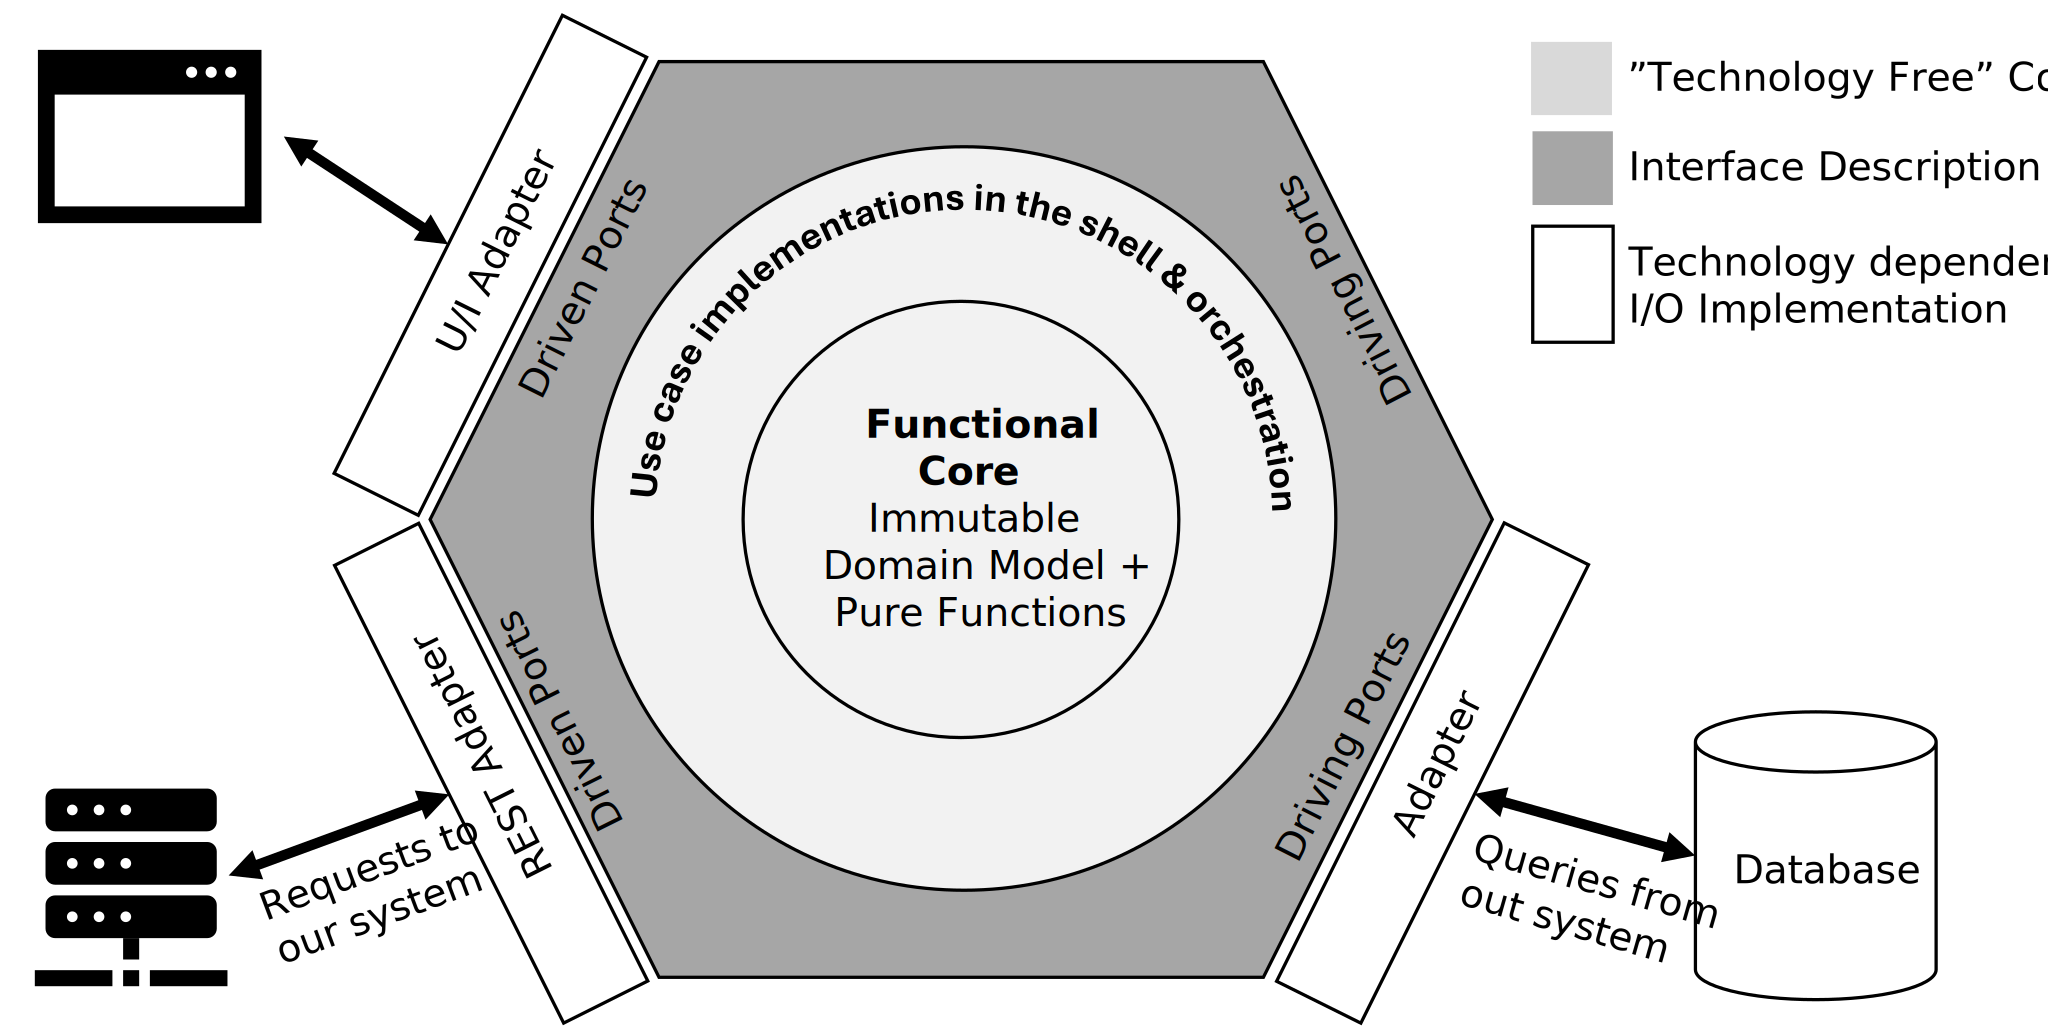
\includegraphics[width=\linewidth]{chapter1/Architecture.pdf}
  \caption{Kombinierte Darstellung der verschiedenen Architekturansätze}
  \label{fig:architecture}
\end{figure}

\section{Die Applikationsschicht}
Am einfachsten verständlich werden diese Architekturkonzepte, wenn man 
sie im Code anwendet. Beginnen wir mit der Definition der Usecases. 
Auch hier ist der Code gleich wieder die Dokumentation. Endlich haben
wir damit auch ein Architekturpattern gefunden in dem sich die Usecases
wirklich auch im Code widerspiegeln. Somit wird die Dokumentation nicht
zur lästigen Pflichtübung sondern ist integraler Bestandteil des Designs,
wie uns Listing \ref{lst:useCases} zeigt:

\begin{listing}[H]
\begin{minted}{java}
public interface ListAllBooksUseCase {
    List<Book> listAllBooks();
}

public interface LookupBookUseCase {
    Optional<Book> lookupIsbn(Isbn isbn);
}

public interface RegisterBookUseCase {
    void register(Book book);
}
\end{minted}
\caption{Die drei UseCases der Applikation}
\label{lst:useCases}
\end{listing}

Usecases sind in diesem Fall einfache Interfaces, die selbsterklärende
Namen haben sollten. Alleine im Verzeichnisbaum kann man so bereits
grob sehen, was die Applikation tut, sprich welche Usecases im Design
vorgesehen wurden.

Zu Demonstrationszwecken implementieren wir diese Usecases in zwei
Service-Klassen. Man hätte auch alles in eine einzige Klasse packen können
aber ich wollte an diesem Punkt die Gestaltungsfreiheit zeigen.

\begin{listing}[H]
\begin{minted}{java}
@Service
public class QueryBooksService implements ListAllBooksUseCase, LookupBookUseCase {

    private final BookPersistence findBook;

    public QueryBooksService(BookPersistence findBook) {
        this.findBook = findBook;
    }

    @Override
    public List<Book> listAllBooks() {
        return findBook.findAll();
    }

    @Override
    public Optional<Book> lookupIsbn(Isbn isbn) {
        return findBook.findBy(isbn);
    }
    
}
\end{minted}
\caption{Implementierung der ListAll- und Lookup Usecases}
\label{lst:lookupUseCase}
\end{listing}

Zugegeben, listing \ref{lst:lookupUseCase} sieht leer und redundant aus. 
Die Anfragen werden einfach durchgereicht. Das liegt aber mehr an der 
Trivialität unserer Applikation als an der Architektur. Aber ist das nicht
grossartig, wie sich die erste Zeile bereits liest? Da steht ja fast in 
lesbarem Englisch "Die Klasse QueryBooksService implementiert die beiden
Usecases ListAllBooks und LookupBook". Mehr müssen wir gar nicht wissen.

Was wir noch nicht besprochen haben ist, wo die BookPersistence auf einmal
herkommt. Hier kommen die \textit{driving ports} oder \textit{out ports} ins
Spiel. Da wir uns noch innerhalb unseres Hexagons befinden dürfen wir uns 
noch nicht auf eine spezielle Implementierung festlegen - insofern ist das
ebenfalls ein Interface (Listing \ref{lst:bookPersistence}).

\begin{listing}[H]
\begin{minted}{java}
public interface BookPersistence {
    List<Book> findAll();
    Optional<Book> findBy(Isbn isbn);
    void save(Book book);
}
\end{minted}
\caption{BookPersistence outbound Port}
\label{lst:bookPersistence}
\end{listing}

Die Zweite Service-Klasse ist übrigens zumindest etwas interessanter, da
sie fachliche Logik widerspiegelt (Listing \ref{lst:RegisterBookService}).
An dieser Stelle haben wir festgelegt, dass ein Buch nicht persistiert werden
darf, fall ein anderes Buch bereits mit dieser ISBN registriert ist.

\begin{listing}[H]
\begin{minted}{java}
@Service
public final class RegisterBookService implements RegisterBookUseCase {

    private final BookPersistence bookPersistence;

    public RegisterBookService(
            BookPersistence bookPersistence
    ) {
        this.bookPersistence = bookPersistence;
    }

    @Override
    public void register(Book book) {
        if (bookPersistence.findBy(book.isbn()).isPresent()) {
            throw new IllegalStateException(
                "Book with ISBN " + book.isbn().value() + " already exists"
            );
        }
        bookPersistence.save(book);
    }
}
\end{minted}
\caption{Implementierung des RegisterBook Usecase}
\label{lst:RegisterBookService}
\end{listing}

Man beachte das \textit{@Sercive} über der Klasse. Das wäre eigentlich von der
Architektur her verboten, denn es stellt eine technische Abhängigkeit der
Klasse zu Spring her. Wenn man das sinnvoll argumentieren kann, dann lohnt
sich zuweilen ein gewisser Pragmatismus. So auch in diesem Fall. 
\textit{@Sercive}\ ändert nichts am Verhalten der Komponente und könnte bei der
Portierung einfach gelöscht werden. Bei den Tests haben wir alleine schon 
wegen den späteren Integrations- und Systemtests die Abhängigkeiten zu Spring
auf Projektebene(!) ohnehin. Insofern ändert sich rein gar nichts und wir 
ersparen uns dabei das redundante erstellen von den \textit{Configurers}.
Spring beherrscht Dependency-Injection bereits in nahezu Perfektion.

\subsection{Applikationsschicht - Tests}
Testen ist auch auf der Applikationsschicht notwendig und sinnvoll. Aufgrund
unserer sauberen Architektur können wit aber selbst auf dieser Ebene noch
vollständig auf UnitTests zurückgreifen. Vor allem haben wir an dieser Stelle
beinahe perfekt vorbereitete ``Units'' - es sind unsere Usecases! Das eignet
sich gut, denn das sind ja genau abgegrenzte \textit{units of work}.

Es reicht an dieser Stelle nur einen der Tests zu zeigen, die anderen beiden
funktionieren völlig analog zu Listing \ref{lst:RegisterBookUseCaseTest}.

\begin{listing}[H]
\begin{minted}{java}
public class RegisterBookUseCaseTest {
    
    private static BookPersistence bookPersistence;
    private static RegisterBookUseCase usecase;

    @BeforeEach
    void setup() {
        bookPersistence = new InMemoryBookPersistenceAdapter();
        usecase = new RegisterBookService(bookPersistence);
    }

    @Test
    void registers_book_if_not_existing() {
        var book = new Book(
                new Title("Domain-Driven Design"),
                new Isbn("9780321125217")
        );
        usecase.register(book);
        assertTrue(bookPersistence.findBy(book.isbn()).isPresent());
    }

    @Test
    void rejects_book_with_existing_isbn() {
        var book = new Book(
                new Title("Domain-Driven Design"),
                new Isbn("9780321125217")
        );
        usecase.register(book);
        assertThrows(
                IllegalStateException.class,
                () -> usecase.register(book)
        );
    }
}
\end{minted}
\caption{RegisterBookUseCase Unit Test}
\label{lst:RegisterBookUseCaseTest}
\end{listing}

Damit der Test laufen kann benötigen wir ein funktionierendes Repsoitory.
Man hätte die echte Datenbank nehmen können - aber dann würde es wieder 
zu einem Integrationstest. Allerdings ist unsere Persistenzschicht derart
einfach, dass man sich einfach eine In-Memory-Implementierung schreiben kann:

\begin{listing}[H]
\begin{minted}{java}
public final class InMemoryBookPersistenceAdapter
        implements BookPersistence {

    private final Map<Isbn, Book> store = new HashMap<>();

    @Override
    public Optional<Book> findBy(Isbn isbn) {
        return Optional.ofNullable(store.get(isbn));
    }

    @Override
    public void save(Book book) {
        store.put(book.isbn(), book);
    }

    @Override
    public List<Book> findAll() {
        return store.values().stream().toList();
    }
}

\end{minted}
\caption{InMemoryBookPersistenceAdapter}
\label{lst:InMemoryBookPersistenceAdapter}
\end{listing}

Mehr als in Listing \ref{lst:InMemoryBookPersistenceAdapter} braucht es gar 
nicht, damit wir testen können. 
Somit sind wir fertig und fügen dem Projekt auf dieser Schicht folgende
Files hinzu:

\dirtree{%
.1 srcPackageRoot/.
.2 application/.
.3 port/.
.4 in/.
.5 ListAllBooksUseCase.java/.
.5 LookupBookUseCase.java/.
.5 RegisterBookUseCase.java/.
.4 out/.
.5 BookPersistence.java/.
.3 service/.
.4 QueryBooksService.java/.
.4 RegisterBookService.java/.
.1 testPackageRoot/.
.2 adapters/out/memory/.
.3 InMemoryBookPersistenceAdapter.java/.
.2 application/.
.3 ListAllBooksUseCase.java/.
.3 LookupBookUseCase.java/.
.3 RegisterBookUseCase.java/.
}%

Somit ist unser Applikationskern fertig. Mit 25 Java-Files und 685 Zeilen 
Code haben wir einen sehr sauberen Applikationskern erstellt, dessen 3 
Usecases mit 16 Tests überprüft wurden. Das ist natürlich ein grosser Schritt
von den 137 Zeilen des trivialen Codes, der zudem noch die ganze REST- und 
Persistenzanbindung enthielt. Das ist jedoch genau der Preis, den man in Bezug
auf architektonische Excellenz und sauberen Tests bezahlt. Anzahl von Zeilen
Code waren eben noch nie ein guter Prädiktor für die Qualität oder der 
Verständlichkeit einer Software. Aber nun wollen wir den Rest der Applikation
noch vervollständigen.

\section{Adapters}
Im Wesentlichen benötigen wir zwei Adapter, die an unsere Ports andocken.
Einmal den REST-Adapter, der die Schnittstelle nach aussen exponiert und
einemal unseren Pesistenzadapter, der die Anbindung an die Datenbank
implementiert.

\subsection{Persistence Adapter mit JPA}

Der Auftrag ist klar - wir müssen lediglich das Interface BookPersitance aus 
Listing \ref{lst:bookPersistence} implementieren. Das werden wir ziemlich 
Analog zu dem Code aus dem trivialen Beispiel umsetzen.

\begin{listing}[H]
\begin{minted}{java}
@Entity
@Data
@AllArgsConstructor
public class BookEntity {
    @Id
    private String isbn;
    private String title;
}
\end{minted}
\caption{BookEntity mit voller JPA und Lombok-Annotation}
\label{lst:BookEntity}
\end{listing}

In Listing \ref{lst:BookEntity} wird die ISBN direkt als Primärschlüssel
verwendet. Ob das performance-technisch eine gute Idee ist, kommt
darauf an, ob es noch andere Relationen gibt, die auf diesen
Primärschlüssel verweisen. Anderenfalls sollte man doch auf eine
nummerische ID ausweichen.

Um effektiv darauf zugreifen zu können, bneötigen wir noch das passende
Repository (Listing \ref{lst:BookRepository}) was in diesem
Fall leer ist, da wir mit der Standard-Funktionalität auskommen.

\begin{listing}[H]
\begin{minted}{java}
public interface BookRepository extends 
    JpaRepository<BookEntity, String> {
    
}
\end{minted}
\caption{Leeres BookRepository nur mit JPARepository Standardfunktionen}
\label{lst:BookRepository}
\end{listing}

Somit haben wir bereits alle Teile beisammen um den Adapter zu
finalisieren. Es fehlt nur noch seine eigentlich Implementierung,
wie in Listing \ref{lst:JpaBookPersistenceAdapter} gezeigt:

\begin{listing}[H]
\begin{minted}{java}
@Service
public class JpaBookPersistenceAdapter
        implements BookPersistence {

    private final BookRepository bookRepository;

    public JpaBookPersistenceAdapter(BookRepository bookRepository) {
        this.bookRepository = bookRepository;
    }

    @Override
    public Optional<Book> findBy(Isbn isbn) {
        return bookRepository.findById(isbn.value())
                .map(this::toDomain);
    }

    @Override
    public List<Book> findAll() {
        return bookRepository.findAll()
            .stream()
            .map(this::toDomain)
            .toList();
    }

    @Override
    public void save(Book book) {
        bookRepository.save(fromDomain(book));
    }

    private Book toDomain(BookEntity entity) {
        return new Book(
                new Title(entity.getTitle()),
                new Isbn(entity.getIsbn())
        );
    }

    private BookEntity fromDomain(Book book) {
        return new BookEntity(
                book.isbn().value(),
                book.title().text()
        );
    }
}
\end{minted}
\caption{Der JPA Persistenz-Adapter}
\label{lst:JpaBookPersistenceAdapter}
\end{listing}

Nichts davon solle wirklich überraschend sein ausser die beiden privaten
Funktionen \texttt{fromDomain} und \texttt{toDomain}. Da unsere
Entity-Klasse sehr einfach aufgebaut ist und lediglich Strings
benutzt müssen wir zwischen diesen beiden Repräsentationen umwandeln.
Hier sei angemerkt, dass die Umwandlung \texttt{toDomain} bereits
die volle Validierung vornimmt. Wir erinnern uns - ein invalides
Domänenobjekt ist nicht intanziierbar. In gegenrichtung können wir
uns darauf verlassen, dass wir keine invaliden Objekte an die 
Datenbank liefern, da bereits das Interface an die Persistenz
nur über Domänenobjekte definiert wurde. Somit können wir an dieser
Stelle auf weitere Checks verzichten und sind fertig.

Noch ein letzter Hinweis: Persistence ist nur ein Beispiel einer
Service-übergreifender I/O Funktionalität. Logging würde man identisch
mittels eines Ports und eines Adapters implementieren.

\subsection{REST Adapter mit Springboot-web}

Um das Ganze an die Aussenwelt anzubinden müssen wir eine Komponente 
(einen \textit{Adapter}) schreiben, der unsere \textit{driven ports}
entsprechend ansteuert.

\begin{listing}[H]
\begin{minted}{java}
@RestController
@RequestMapping("/api/books")
public class BookController {
    
    private final RegisterBookUseCase registerBookUseCase;
    private final ListAllBooksUseCase listAllBooksUseCase;
    private final LookupBookUseCase lookupBookUseCase;
    
    BookController(
            RegisterBookUseCase registerBook,
            ListAllBooksUseCase listAllBooksUseCase,
            LookupBookUseCase lookupBookUseCase) {
        this.registerBookUseCase = registerBook;
        this.listAllBooksUseCase = listAllBooksUseCase;
        this.lookupBookUseCase = lookupBookUseCase;
    }
    ...
    @GetMapping("/{isbn}")
    ResponseEntity<BookDto> getBook(@PathVariable String isbn) {
        return ResponseEntity.of(
                lookupBookUseCase.lookupIsbn(new Isbn(isbn))
                        .map(this::fromDomain));
    }
    ...
    private BookDto fromDomain(Book book) {
        return new BookDto(
                book.title().text(),
                book.isbn().value());
        }
}
\end{minted}
\caption{REST-Adapter implementiert in BookController.java}
\label{lst:BookController}
\end{listing}

Auch in Listing \ref{lst:BookController} ist die Verwendung der Usecases
erneut sehr schön zu sehen und im Wortlaut zu verstehen. Dieser Controller
steuert die Usecases \textit{RegisterBook}, \textit{ListAllBooks} und
\textit{LookupBook} an. Perfekt - wir wissen sofort um was es geht. An 
dieser Aussenschnittstelle endet auch unsere Domäne. Es wäre ein Zufall,
wenn unsere Aussenwelt die Formate unsere Domäne so 1:1 verwenden könnte.
Daher setzen wir \textit{Data-Transfer-Objects} - oder kurz \textit{DTOs}
ein um den Datenaustausch nach aussen zu beschreiben. Da unser Beispiel
inhaltlich trivial ist, gibt es hier wirklich ein 1:1-Mapping, ausser bei den
Datentypen. Wir bekommen Strings und lifern ein BookDTO 
(Listing \ref{lst:BookDTO}) als record mit Strings
für die Felder. Bei komplexeren Anforderungen ist es auch üblich nach
RequestDTOs und ResponseDTOs zu unterscheiden. So wie es halt von den
Anforderungen her nötig ist. Das Mapping mittels \texttt{fromDomain}
und \texttt{toDomain} kennen wir bereits aus dem Persistenz-Adapter.

\begin{listing}[H]
\begin{minted}{java}
public record BookDto (
        String title,
        String isbn
) {
}
\end{minted}
\caption{BookDTO.java}
\label{lst:BookDTO}
\end{listing}


Zudem legen wir noch eine Konfigurationsklasse an, damit Spring die Exceptions
aus unserem Domain-Model richtig behandelt. In diesem Fall wollen wir nicht
\texttt{500 Internal Server Error} zurückgeben sondern lieber 
\texttt{400 Bad Request} und den Text der Exception als Content zurückliefern.
Ob man so transparent sein möchte ist vor allem eine Securityentscheidung.
Wir machen das einfach mal.

\begin{listing}[H]
\begin{minted}{java}
@ControllerAdvice
public class RestExceptionHandler {

    @ExceptionHandler({
        IllegalArgumentException.class,  
        DomainValidationException.class})
    public ResponseEntity<String> handleBadRequestExceptions(RuntimeException ex) {
        return ResponseEntity
                .status(HttpStatus.BAD_REQUEST)
                .body(ex.getMessage());
    }
}
\end{minted}
\caption{Konfiguration um Exceptions richtig zu behandeln}
\label{lst:RestExceptionHandler}
\end{listing}

\subsection{Adaptertests als Integrationstests}
Damit bleibt nur noch unsere Adapter zu testen. Ob man an dieser Stelle
Unittest benötigt hängt von der Komplexität der Adapter ab. Für unsere
Zwecke genügen an dieser Stelle Integrationstests, da wir eigentlich nur
fachlich langweiliges I/O in diesen Adaptern realisieren. Den Applikationskern
und die Domäne haben wir ja bereits ausführlich getestet.

\begin{listing}[H]
\begin{minted}{java}
@SpringBootTest
@Transactional
public class JpaBookPersistenceAdapterTest {
    
    @Autowired
    JpaBookPersistenceAdapter adapter;

    @Test
    void persists_and_loads_book() {
        Book book = new Book(
                new Title("Effective Java"),
                new Isbn("9780134685991")
        );

        adapter.save(book);
        assertTrue(adapter.findBy(book.isbn()).isPresent());
    }
}
\end{minted}
\caption{Integrationtest des JpaBookPersistenceAdapter}
\label{lst:JpaBookPersistenceAdapterTest}
\end{listing}

Listing \ref{lst:JpaBookPersistenceAdapterTest} zeigt wie einfach wir einen
Integrationstest bewerkstelligen können. Mit \texttt{@SpringBootTest} und
\texttt{@Transactional} starten wir den Springboot-Context und sorgen
dafür dass unsere Testdaten nicht final in die Datenbank geschrieben werden.
Es erfolgt ein \textit{Rollback} am Ende der Testmethode.
Das wäre bei unserer In-Memory-H2-Datenbank zwar unwichtig aber es ist am 
saubersten das gleich so zu spezifizieren.

Final testen wir nun noch unseren REST-Adapter (Listing \ref{}).

\begin{listing}[H]
\begin{minted}{java}
@SpringBootTest
@AutoConfigureMockMvc
@ActiveProfiles("inmemorytest")
@Transactional
class BookControllerTest {

    @Autowired
    MockMvc mockMvc;

    @Autowired
    BookRepository bookRepository;

    @Test
    void registerAndLoadBook() throws Exception {
        mockMvc.perform(post("/api/books")
                .contentType(MediaType.APPLICATION_JSON)
                .content("""
                            {
                              "title": "Effective Java",
                              "isbn": "9780134685991"
                            }
                        """))
                .andExpect(status().isOk());

        mockMvc.perform(get("/api/books"))
                .andExpect(status().isOk())
                .andExpect(jsonPath("$.length()").value(1));

        mockMvc.perform(get("/api/books/9780134685991"))
                .andExpect(status().isOk())
                .andExpect(jsonPath("$.title")
                        .value("Effective Java"));
    }

    @Test
    void testExceptionHandling() throws Exception {
        mockMvc.perform(post("/api/books")
            .contentType(MediaType.APPLICATION_JSON)
            .content("""
                        {
                            "title": "",
                            "isbn": "9780134685991"
                        }
                    """))
            .andExpect(status().is4xxClientError());
    }
}
\end{minted}
\caption{Integrationstest des REST Controllers}
\label{lst:BookControllerTest}
\end{listing}

Damit ist aus Sicht der Entwicklungs- und Testarbeit am Backend alles getan.
In der Aussenschicht um unser Hexagon herum haben wir folgende Dateien dem 
Projekt hinzugefügt:

\dirtree{%
.1 srcPackageRoot/.
.2 adapters/.
.3 in/.
.4 rest/.
.5 BookController.java/.
.5 BookDto.java/.
.5 RestExceptionHandler.java/.
.3 out/.
.4 persistance/.
.5 BookEntity.java/.
.5 BookRepository.java/.
.5 JpaBookPersistenceAdapter.java/.
.1 testPackageRoot/.
.2 adapters/.
.3 in/.
.4 rest/.
.5 BookControllerTest.java/.
.3 out/.
.4 persistence/.
.5 JpaBookPersistenceAdapterTest.java/.
}%

Damit ist das Backend final fertig. Mit 808 Zeilen Code und total 19 
Tests haben wir eine saubere, zukunftssichere sehr verständliche 
Architektur umgesetzt.

\section{Diskussion des Ansatzes}
Natürlich muss man das immer relativieren. Der Ansatz ist für sehr kleine
Projekte sicher ein ``overkill'' und selbst bei grösseren Unterfangen nicht
immer notwendig. Wenn man sich sehr sicher ist, dass der verwendete
Technologiestack sich nicht mehr ändert (also dass man z.B. von 
Springboot und einer relationalen Datenbank nicht abweicht) kann man auch
bewusst eine Abhängigkeit in Kauf nehmen. Ebenso, was den funktionalen Kern
angeht. Es ist eine (zugegeben extrem saubere) Möglichkeit eine 
Domäne in Code abzubilden. Aber wir wissen ja aus unzähligen Projekten davor,
dass es noch viele weitere gute Möglichkeiten gibt dies zu tun. 
Die Lösung, die wir hier angeschaut haben bringt klar mehr Komplexität. Das ist
erst mal schlecht - es kommt jedoch darauf an, welche Form von Komplexität man 
anhäuft (\textit{incidental} vs. \textit{accidental} \textit{complexity}).
Gegen \textit{incidental complexity} kann man nicht viel machen - die passiert
einfach, oder liegt einfach vor. Wenn die modellierte Domäne komplex ist, wird
das automatisch auch komplexeren Code nach sich ziehen (oder zumindest mehr 
Code). Wer jetzt denkt, dass
das Domänenmodell in unserem naiven Code den Sachverhalt viel weniger Komplex 
abbilden konnte, der irrt insofern, als dass das Modell es verpasst hat die 
Komplexität überhaupt abzubilden. Im Endeffekt ist das noch schlimmer - 
erforderliche Komplexität die in Code und Tests ignoriert wird. Das ist 
natürlich ein Problem denn so entsteht fehlerhafte Software. Durch fehlende
Validierung und ein Modell, dass inkonsistente und falsche Repräsentationen
erlaubt entstehen auch schnell echte Sicherheitsprobleme. So oder so, die
Domäne muss schon adäquat abgebildet werden.
Anders sieht es bei der Zwiebel-, hexagonalen oder Ports und Adapter- 
Architektur aus. Je nach Betrachtungsweise ist diese Zerlegung und Abstraktion
genau nicht von der Domäne vorgegeben und motiviert. Das ist allein unsere
Entscheidung, die wir aus Gründen der Testbarkeit, wiederverwendbarkeit, 
Flexibilität der Technologie oder einfach nur zur Aufteilung der Bereiche in
in grossen Teams treffen. Passiert das unüberlegt, dann baut man 
\textit{accidential complexity} auf. Unnötig Komplexität anzuhäufen ist so wie
sonst im Leben Risiken einzugehen ohne einen Ertrag zu erwarten - Eine
dumme Entscheidung!

Um dafür ein besseres Gespür zu erhalten wollen wir eine deutlich
komplexere Domäne Modellieren und ein ganzes System mit Frontend sowie 
technischer Anbindung erstellen um diesen Entscheidungsraum etwas besser 
zu erforschen.

\chapter{Realistischeres Beispiel: PLM für die Elektronikentwicklung}
Nun haben wir das Handwerkszeug, um uns einer realistischeren Domäne
zu widmen. Für diesen Kurs haben wir uns etwas ausgesucht, das auf den ersten 
Blick sehr einfach aussieht, aber bei genauerer Betrachtung viele interessante
Details zum Vorschein bringt. Vermutlich ist das bei den meisten 
nicht-trivialen Domänen nicht anders.

Wir wollen ein System bauen, um elektronische Bauteile zu verwalten, 
katalogisieren und bestellen zu können. Später werden wir das Ganze 
sogar in Design-Werkzeuge (EDA - \textit{Electronic Design Automation})
integrieren und ein Web-Frontend dazu anbieten. Unsere Daten sollen dabei
in einer relationalen Datenbank gespeichert werden. Eine klassische
Business-Applikation also.

Die Sachlage ist schnell erklärt. Entwickler elektronischer Baugruppen
planen in ihren Designs elektronische Bauteile ein. Wir wollen diese
Komponenten nennen. Das könnte z.B. ein Widerstand mit einem bestimmten Wert
in einem bestimmten Gehäuse sein. Ganz konkret etwa ein 10k-Ohm-Widerstand in
einem 0603-SMD-Package. Auf dieser Ebene ist das erst mal komplett abstrakt - 
hunderte Hersteller würden einem dieses Bauteil liefern können und man 
könnte diese über zahlreiche \textit{Distributoren} bestellen. Vielfach
ist der konkrete Hersteller auch irrelevant - so lange das Bauteil den
Spezifikationen genügt. Viele Betriebe führen daher eigene IPNs
(\textit{Internal Part Number}), um Bauteile dieser Art zu gruppieren.
Welches spezifische bestellbare Teil dann durch das Procurement beschafft wird
ist dem Entwickler egal. Und genau das soll unser System abbilden.
Es soll den Zusammenhang zwischen abstrakt/intern verwendeten Komponenten und
tatsächlich bestellbaren Bauteilen herstellen und deren Metadaten verwalten.
Am Schluss wollen wir dem System eine BOM (\textit{Bill of Material}) übergeben
und daraus automatisch Bestellinformationen erzeugen können. Damit das 
halbwegs übersichtlich bleibt, sollen die Bauteile in Kategorien zusammengefasst
werden. Jede Komponente gehört genau einer Kategorie an, und jede Komponente hat
ein oder mehrere bestellbare Bauteile. Für alle Bauteile geltende 
Spezifikationen (vorerst \textit{Attribute} genannt) auf Ebene der Komponente,
falls alle bestellbaren Bauteile dies gleichermassen erfüllen. Anderenfalls gibt 
es bauteilspezifische Attribute auf ebene der konkret bestellbaren Teile.
Das klingt eigentlich übersichtlich und einfach, die meisten von euch werden
bereits nach diesen paar Zeilen eine recht klare Vorstellung einer passenden
Objektstruktur im Kopf haben. Aber lasst uns das wieder sauber beginnen
mit der Modellierung unserer Domäne.


\section{Funktionales Domänenmodell - Daten}

Genau wie bei unserem Buch beginnen wir uns mit den Elementen unserer Domäne
auseinanderzusetzen. Bevor wir uns fragen, was eine ``Komponente'' im abstrakten
Sinne sein soll, können wir beginnen das zu modellieren, was wir am einfachsten
beschreiben können. Das wäre in unserer Domäne wohl das tatsächlich bestellbare
Bauteil.

Wenn wir wieder fordern wollen, dass unsere Domänenelemente immutable sind,
dann müssen wir unsere Felder wieder in einzelne Datentypen zerlegen. 
In unserem Objekt müssen wir dann wieder nur noch prüfen, dass diese 
nicht null sind. So sähe unser Record aus:

\begin{listing}[H]
\begin{minted}{java}
public record OrderableItem (
    ManufacturerPartNumber mpn,
    StockKeepingUnit sku,
    Distributor distributor,
    Quantity minOrderQuantity,
    Multiplier orderMultiple,
    UnitPrice price,
    List<Attribute> attributes
) {
}
\end{minted}
\caption{OrderableItem als Record-Typ}
\label{lst:recordOrderItemModel}
\end{listing}

Und es müssen auch nicht alles einzelne Werte sein, unsere Typen können 
ihrerseits durchaus auch komposit sein. Unser \texttt{Price}-Typ z.B.
Neben dem nummerischen Wert des Preises gehört auch die Angabe einer 
Währung fest zu diesem Typ. Eine blosse zahl macht hier keinen Sinn, da
man elektronische Teile oft in ausländischen Währungen bezahlt. 
Je nach Anforderungen würde man noch viel mehr Informationen
zum Preis einfordern - z.B. ob mit dieser mit oder ohne Mehrwertsteuer 
angegeben wurde etc. Der Distributor
bräuchte dann evtl. noch Informationen zum Steuersatz, Verzollung, 
Versandkostenpauschalen, etc. Das ist noch beliebig ausbaubar. 
Aber lassen wir das aktuell noch bewusst simpel. Da wir uns ja nun darauf 
verlassen können, dass alle FeldTypen
immer nur valide Ausprägungen beinhalten, müssen wir nur noch dafür sorgen, dass
uns nicht jemand einen Null-Wert setzt. Neben den Null-Checks gibt es noch
eine fachliche Überprüfung. Es kann nicht sein, dass das Order-Multiple grösser
als die Mindestbestellmenge ist. Das wäre jetzt eine Konsistenzprüfung zwischen
den Werten. Dann gibt es am Schluss noch das ``Problem'' mit den Listen-Typen (
Gleiches gilt auch für Sets und Maps etc.) - so wie deklariert, wäre nur die
Referenz auf die Liste immutable, aber noch nicht ihr Inhalt. Das darf natürlich 
nicht sein und wir erzeugen uns daher auf jeden Fall eine Kopie der bestehenden
Liste, die uns übergeben wurde, damit nicht etwa der Aufrufende noch eine 
Referenz darauf halten kann, um die Liste im Nachhinein 
(also nach Verlassen unseres Konstruktors) nochzu manipulieren. 
In diesem Fall tolerieren wir sogar einen Null-Wert und 
ersetzen diesen sofort durch eine leere Liste. Die \texttt{copyOf}-Methode
erzeugt uns übrigens eine read-only-Liste. Da nun sowohl die Referenz als auch die 
Liste als auch die Elemente (weil es alles Domänen-Elemente sind) dieser Liste 
selbst immutable sind, 
ist der gesamte Objektbaum immutable. 

\begin{listing}[H]
\begin{minted}{java}
public record OrderableItem(
        ManufacturerPartNumber mpn,
        StockKeepingUnit sku,
        Distributor distributor,
        Quantity minOrderQuantity,
        Multiplier orderMultiple,
        UnitPrice price,
        List<Attribute> attributes) {

    public OrderableItem {
        if (mpn == null)
            throw new IllegalArgumentException(
                    "An OrderableItem must have a valid MPN");
        if (sku == null)
            throw new IllegalArgumentException(
                    "An OrderableItem must have a valid SKU");
        if (distributor == null)
            throw new IllegalArgumentException(
                    "An OrderableItem must have a valid Distributor");
        if (minOrderQuantity == null)
            throw new IllegalArgumentException(
                    "An OrderableItem must have a valid minOrderQuantity");
        if (orderMultiple == null)
            throw new IllegalArgumentException(
                    "An OrderableItem must have a valid orderMultiple");
        if (orderMultiple.value() > minOrderQuantity.value())
            throw new IllegalArgumentException(
                    "minOrder Quantity cannot be smaller than orderMultiple");
        if (price == null)
            throw new IllegalArgumentException(
                    "An OrderableItem must have a valid Price");
        if (attributes == null)
            attributes = List.of();
        
        attributes = List.copyOf(attributes);
    }
}
\end{minted}
\caption{Vollständig validierter OrderItem Record}
\label{lst:recordValidatedOrderItemModel}
\end{listing}

\texttt{Enums} sind übrigends auch eine hervorragende Möglichkeit, das Modell 
auf gültige
Werte zu beschränken. Nehmen wir z.B. unsere \texttt{Currency}. Im einfachsten
Fall ist das ebenfalls ein simples \texttt{enum}: 

\begin{listing}[H]
\begin{minted}{java}
public enum Currency {
    CHF, EUR, USD
}
\end{minted}
\caption{Currency als simple Enumeration}
\label{lst:currencyEnum}
\end{listing}

Somit können wir nun auch unseren UnitPrice-Record darstellen:

\begin{listing}[H]
\begin{minted}{java}
public record UnitPrice(
    BigDecimal value,
    Currency currency
) {
    public static final BigDecimal MAX_PRICE = new BigDecimal(1000);

    public UnitPrice {
        if(value == null || value.signum() < 0) {
            throw new IllegalArgumentException(
                "A Price must have a positive value");
        }
       
        // We always want to have 4 decimal places in pricing information
        value = value.setScale(4, RoundingMode.HALF_UP);
        
        if(value.compareTo(new BigDecimal("0.0001")) < 0) {
            throw new IllegalArgumentException(
                "A single item price must be >= 0.0001 in any currency");
        }

        if(value.compareTo(MAX_PRICE) > 0) {
            throw new IllegalArgumentException(
                "A single item price must be <= " + MAX_PRICE + " in any currency");
        }
        if(currency == null) {
            throw new IllegalArgumentException(
                "A Price must specify its currency");
        }

    }
}
\end{minted}
\caption{Price-Record mit Validation}
\label{lst:priceRecord}
\end{listing}

Listing \ref{lst:priceRecord} zeigt den Price-Record mit einer Validierung
des Wertebereichs und der Sicherstellung der geforderten Genauigkeit der 
Preisangabe. 4 Nachkommastellen sind nötig, da für kleine Bauteile 
(z.B. Widerstände) die Stückpreise oft weit unterhalb von einem Rappen liegen.
Zu guter Letzt schauen wir uns noch die Validierung der ManufacturerPartNumber an.

\begin{listing}[H]
\begin{minted}{java}
public record ManufacturerPartNumber(
    String value
) {
    public ManufacturerPartNumber {
        if(value == null) 
            throw new IllegalArgumentException(
                "A MPN must not have a null value");
        if(!value.matches("^[0-9a-zA-Z\\-_.:, ]+$"))
            throw new IllegalArgumentException(
                "MPN must match this regexp: \"^[0-9a-zA-Z\\-_.:, ]+$\"");
        value = value.trim();
    }
}
\end{minted}
\caption{ManufacturerPartNumber mit Validation}
\label{lst:mpnRecord}
\end{listing}

Nun wollen wir noch die Attribute in den Griff bekommen. Diese sind gleich in
mehrerer Hinsicht interessant. Erstens müssen sie widerspruchsfrei sein, d.h.
jedes Label darf in jeder Liste auf Ebene der \texttt{OrderableItem} 
und auch der \texttt{Componnet} nur einmal vorkommen. Alleine daran sehen wir,
dass eine \texttt{java.util.Map} die bessere Datenstruktur scheint als eine 
Liste - wenn wir \texttt{AttributeLabel} als \texttt{key} benutzen und 
\texttt{AttributeValue} als \texttt{value} der Map, sind doppelte Einträge
innerhalb einer Map nicht möglich. Lediglich zwischen den Maps müssen wir noch
für Konsistenz sorgen. Wir können sogar noch präziser sein: Ein bestimmtes Label
ist auf Ebene der \texttt{Component} gesetzt und gilt damit für alle 
\texttt{OrderableItem} - nun darf es in den Maps der Items nicht mehr vorkommen.

Aber der Reihe nach. Es geht ja darum, physikalische Grössen in Form einer
Spezifikation in diesen Attributen abzubilden - z.B. eine maximal zulässige
Spannung oder Temperatur, die das Bauteil aushalten muss. Es geht also um 
Messgrössen. Dabei wollen wir auch gleich hinterlegen, ob diese Grössen 
negativ werden können. Listing \ref{lst:quantityEnum} zeigt die Umsetzung mit
einem \texttt{enum}:

\begin{listing}[H]
\begin{minted}{java}
public enum MeasuredQuantity {

    CURRENT(true),
    VOLTAGE(true),
    TEMPERATURE(true),
    POWER(false),
    RESISTANCE(false),
    CAPACITANCE(false),
    INDUCTANCE(false),
    FREQUENCY(false),
    TIME(false),
    LENGTH(false),
    DIMENSIONLESS(true);

    private final boolean allowNegative;

    Quantity(boolean allowNegative) {
        this.allowNegative = allowNegative;
    }

    public void validate(BigDecimal valueInBaseUnit) {
        if (!allowNegative && valueInBaseUnit.signum() < 0) {
            throw new IllegalArgumentException(
                    name() + " must not be negative: " + valueInBaseUnit
            );
        }
    }
}
\end{minted}
\caption{Quantity enum inkl. der Abbildung von Zahlenranges}
\label{lst:quantityEnum}
\end{listing}

Hier zeigt sich auch nochmals, wie leistungsfähig \texttt{enums} in der Praxis
sein können. Neben den Messgrössen benötigen wir noch Einheiten. Auch das ist
nochmals ein \texttt{enum}. In diesem Fall sogar ein noch ausgefeilteres
Vorgehen, da
wir auch gleich noch Informationen zur Umrechnung beifügen wollen. 1000mA sind 
z.B. 1A und 0°C entsprechen 273.15K. Jede Einheit wird dabei einer Messgrösse
zugeordnet.

\begin{listing}[H]
\begin{minted}{java}
public enum Unit {

    VOLT(MeasuredQuantity.VOLTAGE, "V", BigDecimal.ONE, BigDecimal.ZERO),
    MILLIVOLT(MeasuredQuantity.VOLTAGE, "mV", new BigDecimal("0.001"), BigDecimal.ZERO),
    KILOVOLT(MeasuredQuantity.VOLTAGE, "kV", new BigDecimal("1000"), BigDecimal.ZERO),
    
    ...

    KELVIN(MeasuredQuantity.TEMPERATURE, "K", BigDecimal.ONE, BigDecimal.ZERO),
    CELSIUS(MeasuredQuantity.TEMPERATURE, "°C", BigDecimal.ONE, new BigDecimal("273.15"));

    private final MeasuredQuantity quantity;
    private final String symbol;
    private final BigDecimal scaleToBase;
    private final BigDecimal offsetToBase;

    Unit(MeasuredQuantity quantity, String symbol, 
        BigDecimal scaleToBase, BigDecimal offsetToBase) {
            this.quantity = quantity;
            this.symbol = symbol;
            this.scaleToBase = scaleToBase;
            this.offsetToBase = offsetToBase;
    }

    public MeasuredQuantity quantity() {
        return quantity;
    }

    public String symbol() {
        return symbol;
    }

    public BigDecimal toBase(BigDecimal value) {
        return value.multiply(scaleToBase).add(offsetToBase);
    }

    public BigDecimal fromBase(BigDecimal baseValue) {
        return baseValue.subtract(offsetToBase).divide(scaleToBase);
    }
}
\end{minted}
\caption{Gekürzt dargestelltes Unit-enum inkl. Umrechnung in Basiseinheiten}
\label{lst:untiEnum}
\end{listing}

So einen rigiden Ansatz kann man natürlich nur machen, wenn die Elemente der
Domäne absolut stabil bleiben (oder es hinnehmbar ist mit einem Update bis
zum nächsten Release zu warten). Bei uns ist das bis hierhin gegeben - an der
Physik ändert sich in diesem Bereich nicht mehr viel.

Was jetzt noch fehlt sind unsere Labels. Nennen wir sie mal 
\texttt{SpecifiedProperty}. Diesen Properties ordnen wir direkt unsere 
\texttt{Quantities} zu, wie Listing \ref{lst:SpecifiedPropertyEnum} zeigt:

\begin{listing}[H]
\begin{minted}{java}
public enum SpecifiedProperty {

    OPERATING_TEMPERATURE_MIN(MeasuredQuantity.TEMPERATURE),
    OPERATING_TEMPERATURE_MAX(MeasuredQuantity.TEMPERATURE),

    SUPPLY_VOLTAGE_MIN(MeasuredQuantity.VOLTAGE),
    SUPPLY_VOLTAGE_MAX(MeasuredQuantity.VOLTAGE),
    
    POWER_DISSIPATION_MAX(MeasuredQuantity.POWER),

    CLOCK_FREQUENCY_MAX(MeasuredQuantity.FREQUENCY);
    
    ...

    private final MeasuredQuantity quantity;

    ComponentAttribute(Quantity quantity) {
        this.quantity = quantity;
    }

    public Quantity quantity() {
        return quantity;
    }
}
\end{minted}
\caption{Gekürzt dargestelltes SpecifiedProperties-enum}
\label{lst:SpecifiedPropertyEnum}
\end{listing}

Hier könnte man wirklich diskutieren, ob man das nicht lieber mit
Records abbildet um dann flexibler zu sein. Mit diesem Ansatz
wäre hingegen eine parametrische Suche (wie etwa ``gib mir alle Bauteil
mit jeder eigenschaft in jenem Bereich'') einfacher umzusetzen.

Nun können wir alles zusammenfügen und endlich unsere Attribute verwalten. Da es
mehr als nur irgendwelche Attribute sind, wollen wir einen Typ 
\texttt{SpecificationItem} erstellen.
Das implementieren wir mit einem record, der die Eigenschaft (samt Einheit), 
den eigentlichen Wert sowie die Messgrösse speichert. An diesem Punkt können
(und müssen) wir wieder vollständig validieren. Dieses Tripplet darf weder
null-Elemente beinhalten noch darf die Messgrösse mit der Eigenschaft
inkompatibel sein und ausserdem muss der Wertebereich zur Messgrösse passen.

\begin{listing}[H]
\begin{minted}{java}
public record SpecificationItem(
        SpecifiedProperty property,
        BigDecimal value,
        Unit unit) {
    public SpecificationItem {
        if (property == null)
            throw new IllegalArgumentException(
                    "A SpecificationItem must have a property");
        if (value == null)
            throw new IllegalArgumentException(
                    "A SpecificationItem must have a value");
        if (unit == null)
            throw new IllegalArgumentException(
                    "A SpecificationItem must have a unit");
        if (unit.quantity() != property.quantity()) {
            throw new IllegalArgumentException(
                    "Unit " + unit + " does not match Quantity " + property.quantity());
        }
        BigDecimal baseValue = unit.toBase(value);
        property.quantity().validate(baseValue);
    }

    public BigDecimal valueInBaseUnit() {
        return unit.toBase(value);
    }
}
\end{minted}
\caption{Implementierung des SepcificationItem-Record inkl. Validierung}
\label{lst:SpecifiedPropertyEnum}
\end{listing}

Die Früchte unserer Arbeit erkennen wir spätestens, wenn wir eine Komponenten
von Hand instanziieren wollen.

\begin{listing}[H]
\begin{minted}{java}
Component c = new Component(
    new InternalPartNumber("SMD_R_0603_10k"),
    Category.RESISTORS,
    List.of(
        new OrderableItem(
            new ManufacturerPartNumber("RC0603FR-0710KL"),
            new StockKeepingUnit("2421850"),
            new Distributor("Farnell"),
            new Quantity(10),
            new Multiplier(10),
            new UnitPrice(
                new BigDecimal("0.0058"),
                Currency.CHF),
            Map.of(
                SpecifiedProperty.OPERATING_TEMPERATURE_MAX,
                new SpecificationItem(
                    SpecifiedProperty.OPERATING_TEMPERATURE_MAX,
                    new BigDecimal(155), 
                    Unit.CELSIUS),
                SpecifiedProperty.OPERATING_TEMPERATURE_MIN,
                new SpecificationItem(
                    SpecifiedProperty.OPERATING_TEMPERATURE_MIN,
                    new BigDecimal(-55), 
                    Unit.CELSIUS)))),
    Map.of());

\end{minted}
\caption{Manuelle Instanziierung einer Komponente}
\label{lst:manualComponentInstantiation}
\end{listing}

Auch ohne, das wir in die Implementierung schauen müssen ist, dieses Stück
Code in sich lesbar und verständlich. Und wir können uns blind darauf verlassen,
dass wir keine strukturellen Fehler gemacht haben, denn sonst wird das Objekt 
erst gar nicht erzeugt. Wir wissen, dass alles vorhanden und entlang der 
spezifizierten Regeln in sich konsistent ist.

\section{Funktionales Domänenmodell - Unit testing}
Beim Testen haben wir nun gleich zwei Vorteile. Ersten werden wir weniger Test
brauchen, da der Aufgabenbereich des Domänen-Modells viel kleiner geworden ist.
Wir können weder grossartig Konsistenzprobleme erzeugen noch kämen wir mit der
Welt der Datenbanken oder anderer Schnittstellen in Berührung. Was die 
Validierung angeht könnten wir für alles und jedes einen Unit-Test schreiben
aber viel bringen würde das nicht. Was nutzt es die Funktionalität einer
if-then-throw Anweisung zu prüfen? Dass man wirklich alle Elemente des Records
auf \texttt{null} prüft kann auch mittels Inspektion geprüft werden. Wenn man 
da etwas übersieht, würde es einem wahrscheinlich auch beim Schreiben des Tests
nicht auffallen - insbesondere wenn die gleiche Person den Code und den Test
schreibt. Das muss man selbst entscheiden, und ist auch teils Geschmacksache,
TDD-Puristen würden das sicher anders sehen. Damit niemand zu kurz kommt habe
ich versucht möglichst vollständige Tests zu erzeugen.

Bei komplexeren Validierungen scheinen Test hingegen wertvoller. Bei 
Grössenvergleichen vertut man sich schnell mal mit der Reihenfolge im
\texttt{compareTo} oder wundert sich, dass ein \\ \texttt{BigDecimal("10.00")} 
nicht \texttt{equalTo} \texttt{BigDecimal("10")} ist aber \texttt{compareTo()}
dennoch eine \texttt{0} liefert. 
Oder auch bei den String-Validierungen kann man sich schnell
mit den Regexp irren. Das sollten wir daher auf jeden Fall testen. 
Da wir keinerlei Abhängigkeiten zu irgendwelchen Elementen ausserhalb unseres 
Domänenmodells haben und nur Standard-Datentypen benutzen ist praktisch nichts
an Testinfrastruktur notwendig. Und es geht schnell. Auf meinem Laptop laufen
alle 52 Tests für das Domänenmodell insgesamt in etwa einer Sekunde, inklusive
Starten der JVM.

Schauen wir uns zumindest einen dieser Tests mal an:

\begin{listing}[H]
\begin{minted}{java}
class StockKeepingUnitTest {

    @Test
    void nullValueIsRejected() {
        assertThrows(IllegalArgumentException.class,
                () -> new StockKeepingUnit(null));
    }

    @Test
    void invalidCharactersAreRejected() {
        assertThrows(IllegalArgumentException.class,
                () -> new StockKeepingUnit("SKU#001"));
    }

    @Test
    void validValueIsAccepted() {
        StockKeepingUnit sku = new StockKeepingUnit("SKU-001_A");
        assertEquals("SKU-001_A", sku.value());
    }

    @Test
    void valueIsTrimmed() {
        StockKeepingUnit sku = new StockKeepingUnit("  SKU-001  ");
        assertEquals("SKU-001", sku.value());
    }
}
\end{minted}
\caption{UnitTest für die StockKeepingUnit-Klasse}
\label{lst:skuTestcase}
\end{listing}

Wie wir sehen prüfen wir in Listing \ref{lst:skuTestcase} im Wesentlichen
ob unsere Validierungen im Konstruktor wie vorhergesehen funkionieren.
Entweder müssen Exceptions geworfen werden oder wir überprüfen ob die
Werte entsprechend unseren Wünschen gesetzt wurden.

Das ist auf Stufe des Domainmodells bereits alles - zumindest solange wir nur
das Datenmodell anschauen. Nun können wir uns daran machen das erste Stück
Funktionalität bereitzustellen.

\section{Funktionales Domänenmodell - Services}
So lange wir rein funktional (mit puren Funktionen) unterwegs sind, verbietet
sich I/O. Somit gibt es auch keine \texttt{load} oder \texttt{store} Funktionen.

Aber alles was sich mit unserem Domänenmodell abbilden lässt geht wunderbar. 
Bisher hat sich under Datenmodell nur mit den Komponenten an und für sich
beschäftigt. Wir werden noch etwas mehr benötigen, denn wir wollen mit unserem
System ja ausgehend von einem Schaltplan (oder genauer einer Bill-of-Material)
letztlich eine Bestellung erzeugen. Typischerweise möchte man bei einigen
wenigen Distributoren (idealerweise nur bei einem) bestellen, nur hat nicht
immer jeder Distributor alle gewünschten Teile im Angebot. Daher wollen
wir uns als erstes Feature eine Funktion anschauen, die eine Liste von 
Komponenten + Mengenangaben nimmt und uns eine Liste
an Bestellungen (für die einzelnen Distributoren) zurückgibt. Da alle 
Komponenten mindestens ein OrderableItem besitzen muss das immer funktionieren.
Zusätzlich wollen wir der Funktion noch einen preferred Supplier mitgeben.
Der Einfachheit halber verzichten wir momentan auf sämtliche Optimierungen
wie minimaler Preis, minimale Anzahl von Distributoren etc. Wer Spass hat,
kann das gerne als Übung umsetzen.

Was wir zunächst brauchen ist eine Struktur um die BOM abzubilden. Das geht mit
den folgenden beiden Records:

\begin{listing}[H]
\begin{minted}{java}
public record BillOfMaterial(
        List<BillOfMaterialEntry> lines) {

    public BillOfMaterial {
        if (lines == null)
            throw new IllegalArgumentException("A BOM must have an entry list");
        lines = List.copyOf(lines);
        if (lines.size() < 1)
            throw new IllegalArgumentException("A BOM must have at least one entry");
    }
}

public record BillOfMaterialEntry(
        InternalPartNumber ipn,
        Quantity quantity) {

    public BillOfMaterialEntry {
        if (ipn == null)
            throw new IllegalArgumentException("A BOM-Entry must have a valid ipn specified");
        if (quantity == null)
            throw new IllegalArgumentException("A BOM-Entry must have a valid quantity specified");
    }
}
\end{minted}
\caption{Zwei Records um BOMs abzubilden.}
\label{lst:skuTestcase}
\end{listing}

Zusätzlich benötigen wir noch zwei Records um eine Bestellung abzubilden.

\begin{listing}[H]
\begin{minted}{java}
public record Order(
        Distributor distributor,
        List<OrderEntry> lines
) {
    public Order {
        if (distributor == null)
            throw new IllegalArgumentException(
                "An Order must have a valid distributor specified");
        if (lines == null)
            throw new IllegalArgumentException(
                "An Order must have an entry list");
        lines = List.copyOf(lines);
        if (lines.size() < 1)
            throw new IllegalArgumentException(
                "An Order must have at least one entry");
    }
    public Order withLine(OrderEntry line) {
        if (line == null)
            throw new IllegalArgumentException("OrderEntry must not be null");
        List<OrderEntry> copy = new ArrayList<>(lines);
        copy.add(line);
        return new Order(distributor, copy);
    }
}

public record OrderEntry(
        StockKeepingUnit sku,
        ManufacturerPartNumber mpn,
        Quantity quantity) {
    public OrderEntry {
        if (mpn == null)
            throw new IllegalArgumentException(
                "An OrderEntry must have a valid mpn specified");
        if (sku == null)
            throw new IllegalArgumentException(
                "An OrderEntry must have a valid sku specified");
        if (quantity == null)
            throw new IllegalArgumentException(
                "An OrderEntry must have a valid quantity specified");
    }
}
\end{minted}
\caption{Zwei Records um Bestellungen abzubilden.}
\label{lst:OrderRecords}
\end{listing}

Im letzten Listing (\ref{lst:OrderRecords})sieht man auch gut, wie man ein 
Listen-Element eines immutable objects um einen Eintrag erweitert.
Man tut das eben nicht sondern erzeugt ein neues, immutable object, das den
neuen Eintrag additional beinhaltet. Das alte Objekt bleibt wie es ist.

Wem das ungewohnt erscheint, der erinnere sich daran, wie er/sie
seit jeher mit String umgegangen ist. Auch Strings sind in Java schon immer
immutable gewesen. Darum gibt String.replace einen neuen String zurück und 
mutiert den gegeben String eben genau nicht.

Damit ist alles vorbereitet, damit wir unseren ersten Service schreiben können:
\begin{listing}[H]
\begin{minted}{java}

public class OrderService {

    public static List<Order> generateOrders(
            BillOfMaterial bom,
            Map<InternalPartNumber, Component> componentMap,
            Distributor preferredDistributor) {

        Map<Distributor, Order> orderMap = new HashMap<>();
        for (BillOfMaterialEntry bomEntry : bom.lines()) {
            Component component = componentMap.get(bomEntry.ipn());
            if (component == null) 
                throw new IllegalArgumentException(
                    "All BOM-IPNs must be present in the component map");
            /*  Since having at least one orderableItem is an invariant
                we can search the list to find the preferred supplier.
                If that is not present, we fall back to the first one 
                specified. */
            OrderableItem orderableItem = component.orderableItems().stream()
                    .filter(item -> item.distributor().equals(preferredDistributor))
                    .findFirst()
                    .orElse(component.orderableItems().get(0));
            Distributor distributor = orderableItem.distributor();
            OrderEntry entry = new OrderEntry(
                    orderableItem.sku(),
                    orderableItem.mpn(),
                    bomEntry.quantity());
            Order existing = orderMap.get(distributor);
            Order updated = (existing == null)
                    ? new Order(distributor, List.of(entry))
                    : existing.withLine(entry);
            orderMap.put(distributor, updated);
        }
        return List.copyOf(orderMap.values());
    }
}
\end{minted}
\caption{OrderService mit generateOrders als \textit{pure function}}
\label{lst:oserServicepure}
\end{listing}

Alles was wir in Listing \ref{lst:oserServicepure} machen ist schrittweise 
durch die BOM zu iterieren und 
Stück für Stück die Bestellungen zu befüllen, die wir uns in einer Map halten.
Dadurch können wir elegant auch mit mehreren Distributoren gleichzeitig umgehen.
Am Schluss geben wir nur noch die Inhalte der Map zurück und sind fertig.

Wir erwarten vom Aufrufendem Code, dass er uns passend zur BOM eine Map
mit den relevanten Komponenten bereitstellt. Das wird später eine
Datenbankabfrage benötigen. Dennoch können wir die innere Logik völlig losgelöst
davon mit einfachen Unit-Test überprüfen. Genau wie bei den Domänen-Objekten
müssen wir auch hier nur für den passenden Input sorgen so dass wir alle
Pfade einmal ablaufen, wenn wir mit 100\% path-coverage testen wollen. An
dieser Stelle erreichen wir beides. Einerseits ist das eine
\textit{pure function} - somit ohne I/O und ohne Seiteneffekte und andererseits
ausschliesslich von den Datenstrukturen der Domain abhängig.

\section{Applikation und Use-Cases}
Nachdem die Domäne an und für sich abgebildet ist können wir beginnen
die Usecases abzubilden. Das geht in diesem (trotzdem noch immer)
einfachen Fall ganz gut, in grösseren Projekten wird dies wohl eher
ein iterativer Prozess. Für dieses System sind 6 Usecases vorgesehen - 
3 Stück für das Frontend, sowie 3 weitere für die Anbindung an das EDA
System (Listing \ref{lst:labstackUseCases}):

\begin{listing}[H]
\begin{minted}{java}
public interface ListAllComponentsUseCase {
    List<Component> invokeListAllComponents();
}

public interface RetrieveComponentInfoUseCase {
    Component invokeRetrieveComponent(InternalPartNumber ipn);
}

public interface AddOrderableItemUseCase {
    Component invokeUcAddItem(InternalPartNumber internalPartNumber, 
        OrderableItem orderableItem);
}

public interface EDAListCategoriesUseCase {
    List<Category> invokeEDAListCategories();
}

public interface EDAListCetegoryEntriesUseCase {
    List<Component> invokeEDAListCategories(Category category);
}

public interface EDAAccessPartDetailsUseCase {
    Component invokeEDAPartDetails(InternalPartNumber ipn);
}
\end{minted}
\caption{6 Usecases als Interfaces modelliert (\textit{Driven Ports})}
\label{lst:labstackUseCases}
\end{listing}

An dieser Stelle auch nochmals unbedingt der Hinweis, dass wir die Use Cases
aus Sicht der Domäne spezifizieren. Hier geht es explizit noch nicht um
Datenformate für die Präsentation nach aussen hin. Das gilt sowohl für den
Input, als auch für den Output. Man mag versucht sein, die einzige Methode
den Use Cases direkt \texttt{invoke} zu nennen aber davon ist abzusehen.
Sobald ein Service mehrere Dieser Use Cases implementiert, müssten die
Methoden strikt eine unterschiedliche Signatur aufweisen, was nicht immer
gegeben sein muss. Für die Les- und Debugbarkeit ist das auch nicht förderlich.

Das schöne an dieser Vereinzelung ist, dass ein einziger Blick in das
Source-Code-Repository verrät was das System macht, bzw. welche Use Cases es
implementiert:
\\
\dirtree{%
.1 srcPackageRoot/.
.2 application/.
.3 port/.
.4 in/.
.5 AddOrderableItemUseCase.java/.
.5 EDAAccessPartDetailsUseCase.java/.
.5 EDAListCategoriesUseCase.java/.
.5 EDAListCategoryEntriesUsecase.java/.
.5 ListAllComponentsUseCase.java/.
.5 RetrieveComponentInfoUseCase.java/.
}%

Um diese Use Cases zu implementieren werden wir I/O benötigen. Dazu werden
folgende Port-Implementierungen ausserhalb des Hexagons verlangt 
(Listing \ref{lst:drivingPorts}):

\begin{listing}[H]
\begin{minted}{java}
public interface LoggingAdapter {
    void debug(String message);
    void info(String message);
    void warn(String message);
    void error(String message);
}

public interface StoragePersistanceAdapter {
    public void persistNewCompnent(Component component);
    public void updateComponent(InternalPartNumber original, Component replacement);
    public Optional<Component> loadComponent(InternalPartNumber ipn);
    public List<Component> loadAllByCategory(Category category);
    public List<Component> loadAll();
    public List<Category> availableCategories();
}
\end{minted}
\caption{I\/O Ports zur Aussenwelt (\textit{Driving Ports})}
\label{lst:drivingPorts}
\end{listing}

Durch dieses Vorgehen lässt wich jegliches I/O aus dem inneren unseres Hexagons
Isolieren. Innerhalb des Domänen-Kerns würden wir aber nicht mal dieses Angebot
nutzen - dieser soll ja \textit{pure} bleiben. Auf der Schicht aussenrum werden
hingegen die Usecases implementiert. An diesem Punkt ist I/O unumgänglich.


Schauen wir uns dazu exemplarisch die Implementierung 
des AddOrderableItem-Usecase an:
\begin{listing}[H]
\begin{minted}{java}
@Service
public class ComponentsUpdateService implements AddOrderableItemUseCase {

    private final RelationalComponentAdapter relationalComponentAdapter;
    private final LoggingAdapter logger;

    public ComponentsUpdateService(
            RelationalComponentAdapter relationalComponentAdapter, 
            LoggingAdapter logger) {
        this.relationalComponentAdapter = relationalComponentAdapter;
        this.logger = logger;
    }

    @Override
    public Component invokeUcAddItem(InternalPartNumber internalPartNumber,
            OrderableItem orderableItem) {
        // *******************
        // *** Shell: I/O ***
        // *******************
        Component component = relationalComponentAdapter.loadComponent(
                internalPartNumber).orElseThrow(ComponentNotAvailableException::new);

        // *******************
        // *** Pure Core ***
        // *******************
        component = component.withOrderableItem(orderableItem);

        // *******************
        // *** Shell: I/O ***
        // *******************
        relationalComponentAdapter.updateComponent(internalPartNumber, component);
        logger.info("AddOrderableItemUseCase added: " + orderableItem.mpn() 
            + " to Component " + component.ipn() );
        return component;
    }
}

\end{minted}
\caption{Hinzufügen einer Bestelloption zu einem Bauteil}
\label{lst:addOrderable}
\end{listing}

An diesem Beispiel (Listing \ref{lst:addOrderable}) sieht man wie im Pattern
\textit{functional core \& imperative shell} die Trennung zwischen I\/O und
den \textit{pure domain functions} vollzogen wird. Erstens nehmen wir
an dieser Stelle selbst keinerlei I/O vor sondern verwenden dazu vollständig
die Adapter (oder besser gesagt deren Interfaces). In der Mitte dann der
seiteneffektfreie Domain-Code, der aus einer Komponente + neuer Bestelloption
eine neue Komponente erzeugt.

Wie schon im Trivialbeispiel sticht auch hier wieder die Lesbarkeit der 
Signatur der Klasse heraus -
\textit{ComponentsUpdateService implements AddOrderableItemUseCase}. 
Durch den strikten Umweg über die Ports bleiben wir auch auf dieser Ebene
noch vollständig technologiefrei und testbar.

\section{Persistence Adapter}
Genau wie bei dem Trivialbeispiel benötigen wir einen Persistenzadapter zu
unserer Datenbank. Dazu erstellen wir uns Entity-Klassen die die Datenhaltung
der relationalen Datenbank als Objekte Repräsentieren. Es genügt die
Hauptkomponente \texttt{ComponentEntity} anzuschauen:

\begin{listing}[H]
\begin{minted}{java}
@Entity
@Data
@AllArgsConstructor
@NoArgsConstructor
@Builder
public class ComponentEntity {
    
    @Id
    @GeneratedValue(strategy = GenerationType.IDENTITY)
    private Long id;

    @NonNull
    @Column(unique = true)
    private String ipn;

    private String symbolRef;
    
    private String footprintRef;
   
    @Enumerated(EnumType.STRING)
    private Category category;

    @OneToMany(cascade = CascadeType.ALL, orphanRemoval = true)
    @Builder.Default
    private List<OrderableItemEntity> orderableItems = new ArrayList();

    @OneToMany(cascade = CascadeType.ALL, orphanRemoval = true)
    @Builder.Default
    private List<AttributeEntity> attributes = new ArrayList();
}
\end{minted}
\caption{Component Entity}
\label{lst:componentEntity}
\end{listing}

Im Vergleich zum Trivialbeispiel sind hier die Relationen zu anderen
Entities hervorzuheben. Mit \texttt{@OneToMay} bringen wir eine 
\textit{1:N}-Relation zum Ausdruck. Weiter fordern wir, dass 
sowohl die \texttt{OrderableItemEntity}, als auch die 
\texttt{AttributeEntity} vollständig abhängige Entitäten sind,
die sowohl bei Persist als z.B. auch bei Delete mit angelegt oder
entfernt werden. Wir forder sogar, dass es keine nicht-zugeordneten
Entitäten von diesen beiden Typen geben darf. Enums können direkt
aus dem Domänenmodell hinterlegt werden; wie in der Annotation
deklariert, werden sie als Strings auf der Datenbank abgebildet.

Um die Daten in der DB laden und speichern zu können, benötigen wir 
wieder ein JPA-Repository. In diesem Fall kann es nicht leer bleiben:


\begin{listing}[H]
\begin{minted}{java}
public interface ComponentRepository extends JpaRepository<ComponentEntity, Long> {
    Optional<ComponentEntity> findByIpn(String ipn);

    boolean existsByIpn(String ipn);

    List<ComponentEntity> findByCategory(Category category);

    void deleteByIpn(String ipn);

    @Query("SELECT DISTINCT c.category FROM ComponentEntity c")
    List<Category> findDistinctCategories();
}
\end{minted}
\caption{Component Repository}
\label{lst:componentRepository}
\end{listing}

In Listing \ref{lst:componentRepository} haben wir die Standard-Funktionen
wie \textit{findById, save, deleteByID, usw.} das würde für unsere Zwecke
aber nicht genügen. Aus Performance-Gründen haben wir eine numerische ID,
die wir aber ausserhalb der Datenbank gar nicht verwenden. Unsere
Domänenobjekte kennen diese ID nicht, denn es ist ein rein fachliches
Artefakt, das nichts mit der Domäne zu tun hat. Genau an solchen Beispielen
sehen wir die konzeptuellen Vorteile eines Domänengetriebenen Ansatzes.
So lassen wir überhaupt nicht zu, dass unsere Domänemodelle von
technische Randbedingungen kontaminiert werden. Damit wir unsere Komponenten
finden und nach Kategorien ordnen können. Das Interface zeigt hier beide 
Möglichkeiten Queries zu spezifizieren. Einmal über eine strikte
Namenskonvention der Interfaces (nachzulesen in \cite{spring_2026_repo}), 
einmal über die Angabe der Query in JPQL (Spezifikation unter 
\cite{oracle_2026}).

Somit haben wir alles vorbereitet um unseren Persistenz-Adapter zu erstellen:

\begin{listing}[H]
\begin{minted}{java}
@Service
@AllArgsConstructor
public class RelationalComponentAdapter implements StoragePersistanceAdapter {

    private ComponentRepository componentRepository;

    @Override
    public void persistNewCompnent(Component component) {

        if (componentRepository.existsByIpn(component.ipn().value())) {
            throw new IllegalArgumentException("Component must not yet exist to be saved");
        }

        ComponentEntity ce = fromDomain(component);
        componentRepository.save(ce);
    }
    ...
    private OrderableItemEntity fromDomain(OrderableItem oi) {
        return OrderableItemEntity.builder()
                .mpn(oi.mpn().value())
                .sku(oi.sku().value())
                .distributor(oi.distributor())
                .minOrderQuantity(oi.minOrderQuantity().value())
                .orderMultiple(oi.orderMultiple().value())
                .price(oi.price().value())
                .currency(oi.price().currency())
                .attributes(oi.attributes()
                        .entrySet()
                        .stream()
                        .map(e -> fromDomain(e.getValue()))
                        .collect(Collectors.toList()))
                .build();
    }
    ...
}
\end{minted}
\caption{Persistence Adapter (Klasse nur teilweise dargestellt)}
\label{lst:persistenceAdapter}
\end{listing}

Da wir uns nun ausserhalb unseres Hexagons befinden dürfen wir an dieser Stelle
jeden Technologiebezug haben, den wir uns wünschen. Durch die \texttt{@Service}
Annotation kann Spring die Instanziierung dieser Klasse vornehmen,
mittels \texttt{@AllArgsConstructor} erhalten wir über Lombok einen
Konstruktor, der ein \textit{ComponentRepository} verlangen wird.
Spring verdrahtet uns das automatisch. An dieser Stelle müssen wir auch
zwischen Domänen und Entity-Objekten konvertieren. In diesem Fall passiert das
auf Ebene der Adapterimplementierung. Es hätte aber auch nichts dagegen
gesprochen diese Abbildung in der Entity-Klasse vorzunehmen. Das wäre
angebracht, wenn man diese Transformation in mehreren anderen Klassen bräuchte.
An diesem Punk gelten einfache DRY-Prinzipien.

\section{Integration in ein EDA-System}

Mit dem nächsten Adapter binden wir ein technisches System an unser Backend
an. In diesem Fall ein EDA-System \textit{Electronic Design Automation}, also
im Wesentlichen ein Elektronik-CAD. Für dieses Beispiel nehmen wir 
\textit{KiCad}, das aktuell wohl bekannteste Open-Source EDA. KiCad hat selbst
eine Bauteilbibliothek, kann aber über mehrere Mechanismen und Plugins externe
Bibliotheken einbinden. In grösseren Unternehmen ist es eigentlich die Regel
über ein zentralisiertes Bauteilmanagement zu verfügen. Genau das simulieren
wir und nutzen die Fähigkeit von KiCad, ein REST-Interface anzusprechen.

Der Spezifikation des REST-Interfaces \cite{kicad_http_2026} können wir
entnehmen, dass es im Wesentlichen drei Abfragearten gibt: Welche
Kategorien es gibt, welche Bauteile sich in einer bestimmten Kategorie
befinden und natürlich Details zu einem bestimmten Bauteil abzufragen.

Als Ergebnis wird JSON erwartet. Allerdings mit der Einschränkung, dass alle
Elemente reine Strings sind. KiCad parst und konvertiert das eigenständig,
wir werden auf Seite der Adapter das gleiche tun.

\begin{listing}[H]
\begin{minted}{java}
public record KicadComponentDetail(
            String id,
            String name,
            String description,
            String symbolIdStr,
            String exclude_from_bom,
            String exclude_from_board,
            String exclude_from_sim,
            Map<String, KicadFieldData> fields) {

        public static KicadComponentDetail fromDomain(Component c) {
            return new KicadComponentDetail(
                c.ipn().value(), c.ipn().value(), c.ipn().value(),
                c.symbol().value(), "false", "false", "false",
                Map.of("Value", new KicadFieldData(extractValue(c), "true"),
                    "Footprint", new KicadFieldData(c.footprint().value(), "false")));
        }
        
        private static String extractValue(Component c) {
                Optional<SpecificationItem> nominalItem = c.attributes().entrySet().stream()
                    .filter(e -> e.getValue().property().name().contains("NOMINAL"))
                    .findFirst().map(e -> e.getValue());
                if (nominalItem.isEmpty()) {
                    return c.orderableItems().get(0).mpn().value();
                }
                return nominalItem.get().value() + nominalItem.get().unit().symbol();
        }
}
\end{minted}
\caption{KiCad Adapter (KicadComponentDetail - DTO)}
\label{lst:kicadDetailDTO}
\end{listing}
Im Beispiel schauen wir uns die Abbildung unserer Components in das 
entsprechende KiCad-DTO an (Listing \ref{lst:kicadDetailDTO}).
Da es keinen Rückweg gibt - also wir vom CAD-Programm nie Daten erhalten werden -
ist auch nur die Abbildungsrichtung von der Domäne zu KiCad realisiert. Das
erste ``Problem'' ist, dass KiCad einen eindeutigen Identifier benötigt.
Den realisieren wir über die \textit{Internal Part Number}, die wir ohnehin
für eindeutig erklärt haben. \textit{Name} und \textit{Beschreibung} setzen wir
für unsere Tests vorerst ebenfalls auf unsere IPN. Eine gute Beschreibung des
Bauteils nebst Links zu den Datenblättern könnte man jederzeit im Domainmodell
nachführen. Weitere Werte erwartet KiCad als assioziatives Array - also einer
Map. Footprint und Value sind fixe Feldschlüssel, die KiCad versteht. Die
Bereitstellung eines ``Values'' ist eine kleine Herausforderung. Nicht jedes
Bauteil hat das. Ein Widerstand z.B. hat natürlich einen klaren Wert - 
nämlich seinen Widerstandswert. Ein integrierter Schaltkreis nicht unbedingt.
Hier habe ich mich entschieden, nach \textit{Properties} zu suchen, die
mit \texttt{NOMINAL} beginnen. Ein Bauteil mit Werten sollte so ein 
NOMINAL-Feld bereitstellen. Falls das nicht vorhanden ist, geben wir
die MPN des ersten Suppliers an KiCad weiter. Das ist an diesem Punkt
sicher noch ausbaufähig. Es zeigt aber schön, wie wir uns beim Modellieren
der Domäne (unnötig) eingeschränkt hätten, wenn wir nur von diesem einen
CAD-Produkt ausgegangen wären. Andere CAD-Produkte hätten vielleicht ganz
andere Anforderungen.

Am Schluss wollen wir noch kurz in den REST-Controller schauen.
Überraschungen sollte es nun ja keine mehr geben:

\begin{listing}[H]
\begin{minted}{java}
@RestController
@RequestMapping("/kicad-api/v1")
@AllArgsConstructor
public class KiCadControllerREST {

    private final EDAAccessPartDetailsUseCase accessPartDetailsUseCase;

    ...

    @GetMapping("/parts/{id}.json")
    public ResponseEntity<KicadComponentDetail> part(@PathVariable String id) {
        return ResponseEntity.ok(
            KicadComponentDetail.fromDomain(
                accessPartDetailsUseCase.invokeEDAPartDetails(
                    new InternalPartNumber(id))
                ));
    }

}
\end{minted}
\caption{Ausschnitt des KiCad REST-Controllers}
\label{lst:kicadREST}
\end{listing}

Listing \ref{lst:kicadREST} zeigt nur einen Ausschnitt aus dem REST-Controller
aber die Mechanik ist für alle anderen Endpoints in etwa identisch. Genau wie
für menschliche Akteure steuert auch dieser Controller UseCases an, die unser
Domänenkern bereitstellt. Da wir bereits alles vorbereitet haben ist die 
Methode, die den GET-Request abhandelt entsprechend kurz. Genau wie im 
Trivialbeispiel müssen wir uns an dieser Stelle nicht darum kümmern, ob die
\texttt{id} wirklich existiert. Sollte das nicht der Fall sein, wir unser
Domänenkern eine \texttt{ComponentNotAvailableException} werfen. Dadurch wird
unser REST-Controller mit einer 400-Bad-Request antworten, so wie wir das 
übergreifend konfiguriert haben.

Wenn wir KiCad entsprechend konfigurieren (Hostname, Port und API-Path), dann 
können wir selbst mit unserer kleinen Implementierung wirklich Buteile laden.

\begin{figure}[H]
    \centering
    \includegraphics[width=\textwidth]{./chapter2/KiCAD-Selection.png}
    \caption{Zugriff auf die Bauteilbibliothek via KiCad}
    \label{fig:database}
\end{figure}

\section{Ein einfaches Vanilla-JS Frontend}
Eigentlich soll Frontend-Entwicklung nicht der zentrale Fokus dieses Skripts
sein. Hierzu gibt es unzählige bessere Tutorials und eine nicht abreissende
Flut von immer neuen Ansätzen, Frameworks und Rädern die täglich neu erfunden
werden. Für jeden, der Informatik seriös studiert hat, ist Javascript wohl nach
wie vor eine Zumutung. So schlimm, dass man mit TypeScript versucht hat
einen Überbau zu erzeugen, der dann zu Javascript \textit{transpiliert}.
TypeScript hat Typen, aber die sind (aufgrund der Rückwärtskompatibilität)
wohl mehr als Vorschlag als eine statische und strikte Typisierung zu 
verstehen. Immerhin sind viele gute Ansätze aus TypeScript zu JavaScript
zurück geflossen, so dass wir zumindest ordentliche Modulstrukturen und 
ES6-Klassen erhalten haben.
Hinzu kommen die stetig neuen Frameworks, die meist eines gemeinsam haben:
Eine durch \textit{Node} verwaltete Dependency-Hölle. Es ist nicht ungewöhnlich
dass diese Scripts bereits für Demoapplikationen hunderte Pakete nachladen
von zig verschiedenen Entwicklern. Täglich gibt es überall Bugfixes, teils
mit breaking changes - ein Fixieren aller Versionen scheint aufgrund der 
Bedrohungslage durch Fehler keine gute Idee. Aber vielleicht bin ich zu wenig
Frontendentwickler um dafür Verständnis aufzubringen. Ausserdem darf 
jeder/jede machen, was er/sie will.

Diese Kapitel ist auch weniger meine Vorstellung ``wie es sein soll''
sondern eher wie man zu einem Frontend kommt ohne auf noch mehr 
Technologie einzugehen. Vielleicht schreibe ich irgendwann auch mal
ein Skript über saubere Frontendentwicklung - falls so etwas überhaupt
möglich ist.

Anstelle von grossen Frameworks nehmen
wir daher einfach nichts und bauen trotzdem ein Frontend. Ohne 
Compile-Schritt, ohne Packetierung, ohne Depencency-Hölle. Man kann dieses
Kapitel als Exploration lesen, wie sich Webentwicklung ohne Frameworks nur 
mit WebStandards anfühlt. Am Schluss muss man selbst entscheiden ob das 
für das eigene Projekt ein gangbarer Weg ist. Wahrscheinlich eher nicht ...

In der aktuellen Form ist das - im Gegensatz zu den überlegungen im Backend -
\textbf{NICHT} production-ready und soll auch nicht so verstanden werden.
Mehr ein Denkansatz zum eigenen Evaluieren eines geeigneten Frontends.

Immerhin sind wir durch die Beschränkung auf Web-Standards in hohem Masse
Browserunabhängig und können auch recht sicher sein, dass so ein Frontend
auch in 10+ Jahren noch identisch funktioniert.

\subsection{Projekt-Setup}
Damit wir ein lauffähiges Frontend erhalten können, benötigen wir zuerst
einen Webserver. Spring stellt uns diesen direkt zur Verfügung.
Alle Dateien, die unter \texttt{\_root/src/main/resources/static}
abgelegt wird, wird von Spring direkt per http zur Verfügung gestellt.
Zumindest solange die Dependency \textit{spring-boot-starter-web}
inkludiert ist. Das ist bei uns aufgrund der REST-Schnittstelle aber
sowieso gegeben. Keinen externen Webserver zu verwenden hat hierbei
noch den Vorteil, dass sowohl Back- als auch Frontend von der gleicher
Quelle stammt. Anderenfalls müssten wir uns aktiv um \textit{CORS
- Cross Origin Request Sharing} Gedanken machen. Für die lokale
Entwicklung eine Hürde mehr. Ganz sicher ist die Antwort darauf nicht
die CORS-Protection etwa abzuschalten, so wie man das immer wieder
als Empfehlung liest!

Es ginge tatsächlich gänzlich ohne Dependencies aber wer nicht tagelang
mit CSS basteln will, der nimmt dann doch einfach Bootstrap, damit die
Oberfläche zumindest einigermassen ansehnlich erscheint. Das ist jedoch
nur ein einziges .css file. Das können wir problemlos statisch anbieten.
Unseren Web-Folder strukturieren wir wie folgt:

\dirtree{%
.1 src/main/resources/static/.
.2 3rd-party/.
.3 bootstrap.css.
.3 bootstrap.css.map.
.3 LICENSE.
.2 components/.
.2 lib/.
.3 NPElement.js.
.3 NPRouter.js.
.3 NPService.js.
.2 services/.
.2 app.js.
.2 index.html.
.2 LICENSE.
}%

Unsere \texttt{index.html} ist dabei recht spartanisch. Alles was wir hier
wollen ist, dass boostrap.css geladen wird und wir unser app.js einbinden.


\begin{listing}[H]
\begin{minted}{html}
<!DOCTYPE html>
<html>
    <head>
        <link href="./3rd-party/bootstrap.css" rel="stylesheet">

    </head>
    <body>
        <np-app></np-app>
        <script type="module" src="./app.js"></script>
    </body>
</html>
\end{minted}
\caption{index.html}
\label{lst:indexhtml}
\end{listing}

Ebenfalls recht übersichtlich ist unser \texttt{app.js} 
(Listing \ref{lst:appjs}) aber es verlangt nach ein paar Erklärungen.
Zuerst \texttt{NPElement} oder generell der \textit{NP-}Präfix. Mir ist
nichts besseres eingefallen - ``Nano\&Pico'' soll das heissen. Es sollte
ja möglichst kein sein. Egal, die drei Klassen unter \texttt{lib/} sollen
einfach oft wiederverwendete Funktionen kapseln. \texttt{NPElement} erbt
selbst von \texttt{HTMLElement} was wiederum zum WebStandard gehört.
Eine der zentralen Funktionen ist safeHTML dass uns das \textit{Escapen} 
der String-Literals ermöglicht. Daneben haben wir noch den \texttt{NPRouter}
der einfache Routing-Funktionalitäten zur Navigation bereitstellt.
Wie wir sehen, haben wir nur ganz wenige Routen. Der letzte Eintrag
zeigt auch gleich, wie wir eine Seite mit einem übergebenen Parameter
laden können. Was wir auch noch erklären müssen ist
\texttt{\_getLocalElementNameByID(id)}. In NPElement ist so implementiert
dass alle \texttt{IDs} automatisch mit einer UUID als Prefix versehen werden.
Das ist nötig, da wir auf einen Shadow-DOM verzichten und damit sicherstellen
müssen, dass wir eindeutig auf unsere gekapselten Elemente zugreifen können.
Die genannte Funktion stellt bei der Abfrage dann ebenfalls die korrekte
UUID voran.  

\begin{listing}[H]
\begin{minted}{js}
import { NPElement } from './lib/NPElement.js'
import { HomePage } from './components/pages/HomePage.js'
import { ComponentsPage } from './components/pages/ComponentsPage.js'
import { OrderableItemsPage } from './components/pages/OrderableItemsPage.js'


import { NavBar } from './components/navigation/NavBar.js'
import { NPRouter } from './lib/NPRouter.js';


export class App extends NPElement {

    get template() {
        return this.safeHTML`
            <nav-bar></nav-bar>
            <div id="outlet"></div> 
        `;
    }

    constructor(parameters) {
        super();
        this.render();

        const router = new NPRouter(this._getLocalElementNameByID('outlet'));
        router.define([
                { path: '/', component: () => new HomePage() },
                { path: '/home', component: () => new HomePage() },
                { path: '/components', component: () => new ComponentsPage() },                     
                { path: '/components/:id/orderableItems', 
                    component: (id) => new OrderableItemsPage(id) },           
            ]);

        router.handleInitialLoad();
        router.enableLinkInterception();

        window.router = router;
    }

    render() {
        this.innerHTML = this.template;
    }

}

if (!customElements.get('np-app')) {
    customElements.define('np-app', App);
}
\end{minted}
\caption{app.js}
\label{lst:appjs}
\end{listing}

\texttt{NPRouter.js} und \texttt{NPElement.js} sind mit 130 und 53 Zeilen Code
inkl. Kommentaren übersichtlich klein. Dazu kommen noch 50 Zeilen in 
\texttt{NPService.js}. Das heisst unser Framework weist weniger als 250 Zeilen
Code auf und nimmt uns gleichwohl schon eine Menge Arbeit ab.

\subsection{Anbindung an das Backend}

\texttt{NPService} ist übrigens nur ein Wrapper rund um die Fetch-API so dass
wir bequem auf unser REST-Interface zugreifen können. Listing 
{\ref{lst:servicejs}} zeigt, wie wir das für unser REST-Interface anwenden
können:

\begin{listing}[H]
\begin{minted}{js}
import {NPService} from '../lib/NPService.js'

export class ComponentService extends NPService {
static #instance = null;

  static getInstance() {
    if (!ComponentService.#instance) {
      ComponentService.#instance = new ComponentService();
    }
    return ComponentService.#instance;
  }

  constructor() {
    super('/api/components');
  }

  getAllComponents() {
    return this.request('');
  }

  getComponent(internalPartNumber) {
    return this.request('/' + internalPartNumber);
  }

  addOrderableItem(internalPartNumber, orderableItem) {
    return this.post('/' + internalPartNumber + "/orderableItems", orderableItem);
  }
  
}
\end{minted}
\caption{ComponentService.js}
\label{lst:servicejs}
\end{listing}

Somit ist es ein simpler Wrapper damit wir unsere Objekte im Frontend
abfragen können ohne, dass sich Darstellungs- und Infrastrukturcode
mischen würde.

\subsection{Entwurf der einzelnen Pages}

Exemplarisch schauen wir uns die Liste aller Komponenten an.

\begin{listing}[H]
\begin{minted}{js}
import { NPElement } from '../../lib/NPElement.js';
import { ComponentService } from '../../services/ComponentService.js';

export class ComponentsPage extends NPElement {
  constructor() {
    super();
    this.componentService = ComponentService.getInstance();
    this.render();
    this.loadComponents();
  }

  get template() {
    return this.safeHTML`
      <h1>Available Components</h1>
      <div id="componentList">Loading...</div>
    `;
  }

  render() {
    this.innerHTML = this.template;
  }

  async loadComponents() {
    try {
      const components = await this.componentService.getAllComponents();

      if (!Array.isArray(components)) {
        throw new Error("Books response is not an array");
      }

      this._renderComponents(components);
    } catch (error) {
      this._displayError(`Failed to load components: ${error.message}`);
      console.error('Components loading error:', error);
    }
  }
  ...
}
\end{minted}
\caption{ComponentsPage.js - Teil 1}
\label{lst:componentsPage1}
\end{listing}

Listing \ref{lst:componentsPage1} zeigt uns einen Teil der 
ComponentsPage-Komponents. Im Konstruktor besorgen wir uns
eine Referenz auf den Components-Service und rendern erst
mal einen Placeholder. Das eigentliche Laden der Komponenten erfolgt
Asynchron. Sobald wir alle Komponenten geladen haben, rendern wir
erneut und ersetzen unseren Platzhalter. Wie gesagt kein Shadow-DOM
- wir ersetzen einfach das innerHTML von uns selbst. Da wir von
HTMLElement erben, passt das.

\begin{listing}[H]
\begin{minted}{js}
import { NPElement } from '../../lib/NPElement.js';
import { ComponentService } from '../../services/ComponentService.js';

export class ComponentsPage extends NPElement {
    ...
    
    _renderComponents(components) {
        const container = this._getLocalElementByID('componentList');

        const lines = components.map(
            component => this._createComponentEntry(component)).join('');
        container.innerHTML = this.unsafeHTML`
        <table class="table">
            <thead>
            <tr>
                <th scope="col">Part</th>
                <th scope="col">Category</th>
                <th scope="col">Value</th>
                <th scope="col">Footprint</th>
                <th scope="col">Footprint</th>
            </tr>
            </thead>
            <tbody>
            ${lines}
            <tbody>
        </table>`;
  }
  _createComponentEntry(component) {
    return this.safeHTML`
      <tr>
        <th scope="row">
            <a href="/components/${component.ipn}/orderableItems" data-route>
                ${component.ipn}
            </a></th>
        <td>${component.category}</td>
        <td>${component.value}</td>
        <td>${component.symbol}</td>        
        <td>${component.footprint}</td>        
      </tr>
    `;
  }

  _displayError(message) {
    const container = this._getLocalElementByID('componentList');
    container.innerHTML = this.safeHTML`<p class="text-danger">${message}</p>`;
  }
}
\end{minted}
\caption{ComponentsPage.js - Teil 2}
\label{lst:componentsPage2}
\end{listing}

Im zweiten Teil der Klasse in Listing \ref{lst:componentsPage2} geht es nur
noch um das Rendering der Komponenten. Zu beachten ist die Verwendung von 
\texttt{unsafeHTML} und \texttt{safeHTML}. Da \texttt{safeHTML} alle Tags
in den Daten escapen würde, kann man das nicht verschachtelt aufrufen. Um so
wichtiger ist es hier strikt darauf zu achten, dass niemals Daten vom
Backend in einem unsafe-Block gerendert werden. Anderenfalls würde man hier
Tür und Tor für XSS oder ähnliche Angriffe öffnen. Damit man auch erkunden
kann, wie man etwas zum Server schickt, ist in der Klasse OrderableItemsPage
als Demo vorgesehen, dass man weitere Bestelloptionen zu einer Komponente
hinzufügt. Zum Schluss noch ein Screenshot von unserem Nutzerinterface:


\begin{figure}[H]
    \centering
    \includegraphics[width=\textwidth]{./screenshots/Components.png}
    \caption{Frontend - Listing aller Komponenten}
    \label{fig:components}
\end{figure}

\begin{figure}[H]
    \centering
    \includegraphics[width=\textwidth]{./screenshots/OrderableItems.png}
    \caption{Frontend - Bearbeiten der Lieferoptionen einer Komponente}
    \label{fig:orderableItems}
\end{figure}

Damit ist unser Rundgang durch die Frontend-Welt auch schon beendet.
 Wer jetzt der Meinung ist,
dass das mit Framewoks wie Anguar, Vue oder React alles viel einfacher
ginge der mag sicher Recht haben - für unseren Kurs bleiben wir dennoch
Frameworkless, da wir nicht noch mehr Technologie in den Stack laden
wollten. Ausser XSS prevention passiert bei uns im Frontend nicht viel
Es ist für uns eher ein einfacher Weg Abläufe im Backend auszulösen.




\chapter{Zum Schluss}
Ich hoffe dieses Script hat dazu beigetragen, dass das Java-Wissen etwas
aufgefrischt wurde - oder dass die, die bereits seit Jahren mit Java
entwickelt haben, dennoch etwas mitnehmen konnten, und wenn es nur aus
Architektursicht eine neue Perspektive ermöglicht. Evtl. konnten auf diese
Weise auch ein paar \textit{modernere} Sprachfeatures wie die 
\texttt{records}, Stream-API oder das functional-core-Pattern mitgenommen
werden.

Gerade im Sicherheitsbereich wurden viele Dinge gar nicht thematisiert.
Das war aber ganz bewusst, da wir die Security-Belange ausführlich im
Kurs thematisieren. Das Skript sollte an dieser Stelle nicht redundant werden.
Über was wir auch noch an keinem Punkt gesprochen haben sind die verschiedenen
Deployment-Optionen. Auch das machen wir noch im Kurs.

Wer das Skript bis zum Schluss durchgelesen hat, sollte (zumindest was)
Java angeht, bestens auf den Kurs vorbereitet sein. 

\section{Contribution}
Wer zu dem Sckript etwas beitragen möchte sei herzlich dazu eingeladen.
Es wird über GitHub öffentlich als OER zur Verfügung gestellt und kann
(und soll!) gerne geforked werden. Gerne dürfen auch Issues aufgebommen
oder pull-requests gesendet werden. Für die Vorbereitung unseres Kureses
reicht der Inhalt aktuell aus meiner Sicht aber das Ganze darf sich gerne
auch zu einem eigenständigen Lehrmaterial weiterentwickeln.

Zum Abschluss wünsche ich allen Teilnehmenden viel Spass mit dem Kurs
\textit{CAS Secure Software Design \& Development} and der ZHAW.



\printbibliography[title={Literatur}]

\end{document}

